%%%% main.tex, 2022/08/10, 2.5
%%%% Copyright (C) 2020 Vinicius Pegorini (vinicius@utfpr.edu.br)
%%
%% This work may be distributed and/or modified under the conditions of the
%% LaTeX Project Public License, either version 1.3 of this license or (at your option) any later version.
%% The latest version of this license is in
%%   http://www.latex-project.org/lppl.txt
%% and version 1.3 or later is part of all distributions of LaTeX version
%% 2005/12/01 or later.
%%
%% This work has the LPPL maintenance status `maintained'.
%%
%% The Current Maintainer of this work is Vinicius Pegorini.
%%
%% This work consists of the files utfprpb.cls, utfprpb.tex, and
%% utfprpb-dados.tex.
%%
%% The Current Maintainer of this work is Vinicius Pegorini.
%% Updated by:
%% - Marco Aurélio Graciotto Silva;
%% - Rogério Aparecido Gonçalves;
%% - Luiz Arthur Feitosa dos Santos.
%%
%% This work consists of the files utfpr.cls, main.tex, and
%% variaveis.tex.
%% A brief description of this work is in readme.md.

%% ####################################################
%%
%% >> Atenção - Leia isso antes de usar esse template<< 
%%
%% Esse template foi desenvolvido por professores,  com a intenção de ajudar os alunos com as entregas na biblioteca. Não há uma equipe especializada e dedicada mantendo tal template, mas sim professores trabalhando além das suas funções básicas, que são: ensino, pesquisa e extensão.
%
%% Também os mantenedores deste template não são especializados em LaTeX, muito menos em normas da ABNT. Todos que contribuíram com o template fizeram isso visando deixá-lo o mais próximo possível das normas da ABNT e das regras, anseios e expectativas da biblioteca da UTFPR. É muito importante entender que os desenvolvedores do template não têm relação direta com a biblioteca ou com a ABNT. Ou seja, não são os desenvolvedores do template que ditam as regras e normas dos textos que devem ser entregues à biblioteca.

%%É válido informar também, que como não há uma equipe dedicada e especializada, o tempo para colaborar com o template é curto. Desta forma, pode ser que não sejam empregadas as melhores técnicas, métodos e ferramentas para o desenvolvimento do template. Também pode acontecer do template não atender completamente todos os anseios e exigências da ABNT e da biblioteca, pois por exemplo, muitas regras de redação possuem questões interpretativas. Assim, o template sempre estará em contínua evolução e seria extremamente interessante que as pessoas (alunos,  professores,  técnicos e entusiastas) colaborarem com a evolução do template. Toda ajuda será bem vinda! Isso pode ser feito enviando e-mail para os desenvolvedores, desta forma, assim que possível esses vão tentar melhorar o template.

%%O template é apenas mais uma ferramenta para o desenvolvimento de trabalhos para a biblioteca. Todavia, podem existir outros templates LaTeX. Assim como há templates em outros formatos, que não o LaTeX. O mais importante é que qualquer pessoa, utilizando a princípio qualquer ferramenta, pode desenvolver textos que atendem os requisitos da biblioteca apenas estudando, interpretando e seguindo as regras da UTFPR e da ABNT, que estão disponíveis na página Web da instituição. O template é só um facilitador.

%%Por fim,  é necessário entender que infelizmente o ambiente LaTeX pode ser complexo e gerar resultados distintos dependendo do: sistema operacional,  pacotes LaTeX utilizados,  configurações alteradas, editor utilizado, a forma que está sendo redigida textos, figuras,  etc. Assim não há como garantir que o resultado final será o esperado.  Dito tudo isso,  >>UTILIZE ESSE TEMPLATE POR SUA CONTA E RISCO<<. Os desenvolvedores e colaboradores deste template não se responsabilizam pelo resultado do uso deste template e se eximem de qualquer responsabilidade.

%###################################################


% Luiz - pdfa: inclusão do pdfa
\PassOptionsToPackage{
	pdfa
}{hyperref}

%% Classe e opções de documento
\documentclass[%% Opções
%% -- Opções da classe memoir --
  12pt,%% Tamanho da fonte: 10pt, 11pt, 12pt, etc.
  a4paper,%% Tamanho do papel: a4paper (A4), letterpaper (carta), etc.
  % fleqn,%% Alinhamento das equações à esquerda (comente para alinhamento centralizado)
  % leqno,%% Numeração das equações no lado esquerdo (comente para lado direito)
  oneside,%% Impressão dos elementos textuais e pós-textuais: oneside (anverso) ou twoside (anverso e verso, se mais de 100 p.)
  openright,%% Impressão da primeira página dos capítulos: openright (anverso), openleft (verso) ou openany (anverso e verso)
%% -- Opções da classe abntex2 --
  sumario = abnt-6027-2012,%% Formatação do sumário: tradicional (estilo tradicional) ou abnt-6027-2012 (norma ABNT 6027-2012)
  chapter = TITLE,%% Títulos de capítulos em maiúsculas (comente para desabilitar)
  % luiz - comentar section para ser minusculo
  %section = TITLE,%% Títulos de seções secundárias em maiúsculas (comente para desabilitar)
  % subsection = TITLE,%% Títulos de seções terciárias em maiúsculas (comente para desabilitar)
  % subsubsection = TITLE,%% Títulos de seções quartenárias em maiúsculas (comente para desabilitar),
%% -- Opções da classe utfprpgtex --
  pretextualoneside,%% Impressão dos elementos pré  -textuais: pretextualoneside (anverso) ou pretextualtwoside (anverso e verso)
  fontetimes,%% Fonte do texto: fontetimes (times), fontearial (arial) ou fontecourier (courier)
  % vinculoscoloridos,%% Cores nos vínculos (citações, arquivos, links, url, etc.) (comente para desabilitar)
  semrecuonosumario,%% Remoção do recuo dos itens no sumário (comente para adição do recuo, se estilo tradicional)
  usemakeindex,%% Compilação de glossários e índices utilizando makeindex (comente para desabilitar)
  % legendascentralizadas,%% Alinhamento das legendas centralizado (comente para alinhamento à esquerda)
  %aprovacaoestiloppg,%% Folha de aprovação do programa de pós-graduação no estilo do PPG (comente para estilo padrão)
  pardeassinaturas,%% Assinaturas na folha de aprovação em até duas colunas (comente para em uma única coluna)
  % linhasdeassinaturas,%% Linhas de assinaturas na folha de aprovação (comente para remover as linhas)
%% -- Opções do pacote babel --
  english,%% Idioma adicional para hifenização
  french,%% Idioma adicional para hifenização
  spanish,%% Idioma adicional para hifenização
  brazil,%% Idioma principal do documento (último da lista)
]{utfpr}%% Classe utfpr

% Luiz: pdfa: necessário para criar pdfa
\usepackage[a-3b,mathxmp]{pdfx}[2018/12/22] % você pode escolher entre a-1b, a-2b, a-3b - o template ainda não suporta o a-Xa de 

%%%% configuracoes.tex, 2022/05/02, 2.4a

%% ####################################################
%%
%% >> Atenção - Leia isso antes de usar esse template<< 
%%
%% Esse template foi desenvolvido por professores,  com a intenção de ajudar os alunos com as entregas na biblioteca. Não há uma equipe especializada e dedicada mantendo tal template, mas sim professores trabalhando além das suas funções básicas, que são: ensino, pesquisa e extensão.
%
%% Também os mantenedores deste template não são especializados em LaTeX, muito menos em normas da ABNT. Todos que contribuíram com o template fizeram isso visando deixá-lo o mais próximo possível das normas da ABNT e das regras, anseios e expectativas da biblioteca da UTFPR. É muito importante entender que os desenvolvedores do template não têm relação direta com a biblioteca ou com a ABNT. Ou seja, não são os desenvolvedores do template que ditam as regras e normas dos textos que devem ser entregues à biblioteca.

%%É válido informar também, que como não há uma equipe dedicada e especializada, o tempo para colaborar com o template é curto. Desta forma, pode ser que não sejam empregadas as melhores técnicas, métodos e ferramentas para o desenvolvimento do template. Também pode acontecer do template não atender completamente todos os anseios e exigências da ABNT e da biblioteca, pois por exemplo, muitas regras de redação possuem questões interpretativas. Assim, o template sempre estará em contínua evolução e seria extremamente interessante que as pessoas (alunos,  professores,  técnicos e entusiastas) colaborarem com a evolução do template. Toda ajuda será bem vinda! Isso pode ser feito enviando e-mail para os desenvolvedores, desta forma, assim que possível esses vão tentar melhorar o template.

%%O template é apenas mais uma ferramenta para o desenvolvimento de trabalhos para a biblioteca. Todavia, podem existir outros templates LaTeX. Assim como há templates em outros formatos, que não o LaTeX. O mais importante é que qualquer pessoa, utilizando a princípio qualquer ferramenta, pode desenvolver textos que atendem os requisitos da biblioteca apenas estudando, interpretando e seguindo as regras da UTFPR e da ABNT, que estão disponíveis na página Web da instituição. O template é só um facilitador.

%%Por fim,  é necessário entender que infelizmente o ambiente LaTeX pode ser complexo e gerar resultados distintos dependendo do: sistema operacional,  pacotes LaTeX utilizados,  configurações alteradas, editor utilizado, a forma que está sendo redigida textos, figuras,  etc. Assim não há como garantir que o resultado final será o esperado.  Dito tudo isso,  >>UTILIZE ESSE TEMPLATE POR SUA CONTA E RISCO<<. Os desenvolvedores e colaboradores deste template não se responsabilizam pelo resultado do uso deste template e se eximem de qualquer responsabilidade.

%###################################################

%% Pacotes carregados nas classes:
%%   memoir: abstract, appendix, array, booktabs, ccaption, chngcntr, chngpage, dcolumn, delarray, enumerate, epigraph, framed,
%%           ifmtarg, ifpdf, index, makeidx, moreverb, needspace, newfile, nextpage, parskip, patchcmd, setspace, shortvrb, showidx,
%%           tabularx, titleref, titling, tocbibind, tocloft, verbatim, verse.
%%   memoir (similares): crop, fancyhdr, geometry, sidecap, subfigure, titlesec.
%%   abntex2: babel, bookmark, calc, enumitem, ifthen, hyperref, textcase.
%%   utfprpgtex: abntex2cite, ae, algorithmic, amsmath, backref, breakurl, caption, cmap, color, eepic, epic, epsfig, etoolbox,
%%               fancyhdr, fix-cm, fontenc, glossaries, graphics, graphicx, helvet, hyphenat, indentfirst, inputenc, lastpage,
%%               morewrites, nomencl, sfmath, sistyle, substr, times, xtab.


%% Pacotes adicionais (\usepackage[options]{package})
\usepackage{bigdelim, booktabs, colortbl, longtable, multirow}%% Ferramentas para tabelas
\usepackage{amssymb, amstext, amsthm, icomma}%% Ferramentas para linguagem matemática
\usepackage{pifont, textcomp, wasysym}%% Símbolos de texto
\usepackage{lipsum}				% para geração de dummy text
\usepackage{subfig}             % para adicionar figuras lado a lado no texto                    
\usepackage{pdfpages}           % para adicionar documentos pdf ao trabalho
\usepackage{xspace}


% luiz: primeira letra maiúscula
% solução 1
%\usepackage{stringstrings}
%\newcommand{\firstcap}[1]{\caselower[e]{#1}\capitalize{\thestring}}

% solução 2 - não usei essa
% \usepackage[utf8]{inputenc}
% \usepackage{datatool-base}
% \usepackage{mfirstuc}

% Formatação do título da seção - primeira letra caixa alta e o resto em caixa baixa.
% \usepackage[explicit]{titlesec}
% \usepackage{lipsum}
% \titleformat{\section}{\normalfont}{\thesection}{1em}{\textbf{\firstcap{#1}}} % funciona mas apenas para o título da seção e não para o sumário (a configuração do sumário está mais para baixo

% luiz: define o underline colorido.
% https://github.com/abntex/abntex2-contrib/blob/master/customizacoes/pucminas/abntex2-pucminas.sty
% acabei não usando o black e o coloruline da solução do link

\usepackage[normalem]{ulem} % para o underline colorido na seção quaternária
\renewcommand*{\cftsubsubsectionfont}{\normalfont\uline} % underline no sumário
\setsubsubsecheadstyle{\ABNTEXsubsubsectionfont\ABNTEXsubsubsectionfontsize\ABNTEXsubsubsectionupperifneeded\uline} %underline no título da subsubsection

% luiz: bibliografia - opções

%% Comandos personalizados (\newcommand{name}[num]{definition})
\newcommand{\cpp}{\texttt{C$++$}}%% C++
\newcommand{\latex}{\LaTeX\xspace}%% LaTeX
\newcommand{\ds}{\displaystyle}%% Tamanho normal das equações
\newcommand{\bsym}[1]{\boldsymbol{#1}}%% Texto no modo matemático em negrito
\newcommand{\mr}[1]{\mathrm{#1}}%% Texto no modo matemático normal (não itálico)
\newcommand{\der}{\mr{d}}%% Operador diferencial
\newcommand{\deri}[2]{\frac{\der #1}{\der #2}}%% Derivada ordinária
\newcommand{\derip}[2]{\frac{\partial #1}{\partial #2}}%% Derivada parcial
\newcommand{\pare}[1]{\left( #1 \right)}%% Parênteses
\newcommand{\colc}[1]{\left[ #1 \right]}%% Colchetes
\newcommand{\chav}[1]{\left\lbrace #1 \right\rbrace}%% Chaves
\newcommand{\sen}{\operatorname{sen}}%% Operador seno
\newcommand{\senh}{\operatorname{senh}}%% Operador seno hiperbólico
\newcommand{\tg}{\operatorname{tg}}%% Operador tangente
\newcommand{\tgh}{\operatorname{tgh}}%% Operador tangente hiperbólico
\newcommand{\seqref}[1]{Equação~\eqref{#1}}%% Referência de uma única equação
\newcommand{\meqref}[1]{Equações~\eqref{#1}}%% Referência de múltiplas equações
\newcommand{\citep}[1]{\cite{#1}}%% Atalho para citação implícita
\newcommand{\citet}[1]{\citeonline{#1}}%% Atalho para citação explícita
\newcommand{\citepa}[1]{(\citeauthor{#1})}%% Atalho para citação implícita (somente autor)
\newcommand{\citeta}[1]{\citeauthoronline{#1}}%% Atalho para citação explícita (somente autor)
\newcommand{\citepy}[1]{(\citeyear{#1})}%% Atalho para citação implícita (somente ano)
\newcommand{\citety}[1]{\citeyear{#1}}%% Atalho para citação explícita (somente ano)

\newcommand{\fonteTexto}[1]{\renewcommand{\familydefault}{#1}}

% Define o caminho das figuras
\graphicspath{{figuras/}}

% Define a fonte ara helvet que é uma fonte similar à Arial, se for usar a Arial tem que mudar o compilador para XeLaTex, mas ai tem que arrumar os erros: https://latex.org/forum/viewtopic.php?t=25998
%\usepackage{helvet}
%\renewcommand{\familydefault}{\sfdefault}
%\usepackage{times} % para fonte time new roman
%\usepackage{pslatex} % ou essa aqui...

%\usepackage{titlesec}

%% Configuração de glossário
% \usepackage[portuguese]{nomencl}
% \usepackage[nogroupskip,nonumberlist,nopostdot,nohypertypes={acronym}]{glossaries}
% \makenoidxglossaries
\usepackage{glossaries}
\makeglossaries

% para siglas em português
\newcommand{\siglaPt}[2]
{
 \newglossaryentry{#1}{
  name=#1,
  description={#2},
  first={#2 (#1)},
  long={#2}
 }  
}

% para siglas de língua estrangeira, nessas a descrição longa fica em itálico.
\newcommand{\siglaIt}[2]
{
 \newglossaryentry{#1}{
  name=#1,
  description={\textit{#2}},
  first={\textit{#2} ({#1})},
  long={\textit{#2}}
 }  
}

%% luiz - para fazer os avisos
\usepackage{tcolorbox}

% use para criar caixas de avisos, pode ser utilizado para fazer anotações de tarefas indicadas pelo orientador/banca.
% \caixa{Atenção}{texto...}
\newcommand{\caixa}[2]{
\begin{tcolorbox}[colback=red!5!white,colframe=red!45!white, title = #1, fonttitle=\bfseries]
#2
\end{tcolorbox}
}

% Luiz - Linhas órfãs e viúvas
\widowpenalty=10000
\clubpenalty=10000

% Luiz - Caption do tamanho da Tabela
%\usepackage[width=1\textwidth]{caption}

% Luiz - configurar a margem dos itens
\setlength{\leftmargini}{1.5cm}
\setlength{\leftmarginii}{1.5cm}


%% Arquivo de dados do modelo de documento LaTeX para produção de trabalhos acadêmicos da UTFPR
%%%% variaveis.tex, 2022/05/02, 2.4a
%%%% Copyright (C) 2020 Vinicius Pegorini (vinicius@utfpr.edu.br)
%%
%% This work may be distributed and/or modified under the conditions of the
%% LaTeX Project Public License, either version 1.3 of this license or (at your
%% option) any later version.
%% The latest version of this license is in
%%   http://www.latex-project.org/lppl.txt
%% and version 1.3 or later is part of all distributions of LaTeX version
%% 2005/12/01 or later.
%%
%% This work has the LPPL maintenance status `maintained'.
%%
%% The Current Maintainer of this work is Vinicius Pegorini.
%% Updated by:
%% - Marco Aurélio Graciotto Silva;
%% - Rogério Aparecido Gonçalves;
%% - Luiz Arthur Feitosa dos Santos.
%%
%% This work consists of the files utfpr.cls, main.tex, and
%% variaveis.tex.
%%
%% A brief description of this work is in readme.txt.

%% ####################################################
%%
%% >> Atenção - Leia isso antes de usar esse template<< 
%%
%% Esse template foi desenvolvido por professores,  com a intenção de ajudar os alunos com as entregas na biblioteca. Não há uma equipe especializada e dedicada mantendo tal template, mas sim professores trabalhando além das suas funções básicas, que são: ensino, pesquisa e extensão.
%
%% Também os mantenedores deste template não são especializados em LaTeX, muito menos em normas da ABNT. Todos que contribuíram com o template fizeram isso visando deixá-lo o mais próximo possível das normas da ABNT e das regras, anseios e expectativas da biblioteca da UTFPR. É muito importante entender que os desenvolvedores do template não têm relação direta com a biblioteca ou com a ABNT. Ou seja, não são os desenvolvedores do template que ditam as regras e normas dos textos que devem ser entregues à biblioteca.

%%É válido informar também, que como não há uma equipe dedicada e especializada, o tempo para colaborar com o template é curto. Desta forma, pode ser que não sejam empregadas as melhores técnicas, métodos e ferramentas para o desenvolvimento do template. Também pode acontecer do template não atender completamente todos os anseios e exigências da ABNT e da biblioteca, pois por exemplo, muitas regras de redação possuem questões interpretativas. Assim, o template sempre estará em contínua evolução e seria extremamente interessante que as pessoas (alunos,  professores,  técnicos e entusiastas) colaborarem com a evolução do template. Toda ajuda será bem vinda! Isso pode ser feito enviando e-mail para os desenvolvedores, desta forma, assim que possível esses vão tentar melhorar o template.

%%O template é apenas mais uma ferramenta para o desenvolvimento de trabalhos para a biblioteca. Todavia, podem existir outros templates LaTeX. Assim como há templates em outros formatos, que não o LaTeX. O mais importante é que qualquer pessoa, utilizando a princípio qualquer ferramenta, pode desenvolver textos que atendem os requisitos da biblioteca apenas estudando, interpretando e seguindo as regras da UTFPR e da ABNT, que estão disponíveis na página Web da instituição. O template é só um facilitador.

%%Por fim,  é necessário entender que infelizmente o ambiente LaTeX pode ser complexo e gerar resultados distintos dependendo do: sistema operacional,  pacotes LaTeX utilizados,  configurações alteradas, editor utilizado, a forma que está sendo redigida textos, figuras,  etc. Assim não há como garantir que o resultado final será o esperado.  Dito tudo isso,  >>UTILIZE ESSE TEMPLATE POR SUA CONTA E RISCO<<. Os desenvolvedores e colaboradores deste template não se responsabilizam pelo resultado do uso deste template e se eximem de qualquer responsabilidade.

%###################################################

%% Documento
%% Luiz: Define a fonte do texto da monografia
\fonteTexto{\sfdefault} % utilize \rmdefault para Times New Roman ou \sfdefault para Arial
\TipoDeDocumento{Trabalho de Conclusão de Curso de Graduação}%% Tipo de documento: "Tese", "Dissertação" ou "Trabalho de Conclusão de Curso de Graduação", "Estágio Supervisionado"
\NivelDeFormacao{Bacharelado}%% Nível de formação: "Doutorado", "Mestrado", "Bacharelado" ou "Tecnólogo" - ATENÇÃO, isso será utilizado para alterar a formatação do trabalho, pois pode haver formatações distintas dependendo o nível/tipo de trabalho.


%% luiz
% Template LaTex criado pelo Departamento Acadêmico de Computação (DACOM)
% da Universidade Tecnológica Federal do Paraná - Campus Campo Mourão (UTFPR-CM)
% Criado e alterado pelos professores:
% - Marco Aurélio Graciotto Silva
% - Rogério Aparecido Gonçalvez
% - Luiz Arthur Feitosa dos Santos
% Esse template utiliza a licença CC BY:
% Esta licença permite que outros distribuam, remixem, adaptem e criem a partir deste trabalho, mesmo para fins comerciais, desde que atribuam o devido crédito pela criação original.
% https://creativecommons.org/licenses/by/4.0/deed.pt_BR

% Dados do curso. Caso seja BCC:
\program{Curso de Bacharelado em Sistemas De Informação}
\programen{Undergradute Program in Information Systems}
\degree{Bacharel}
\degreearea{Sistemas De Informação}
% Caso seja TSI:
% \program{Curso Superior de Tecnologia em Sistemas para Internet}
% \programen{Undergradute Program in Tecnology for Internet Systems}
% \degree{Tecnólogo}
% \degreearea{Tecnologia em Sistemas para Internet}


% Dados da disciplina. Escolha uma das opções e a descomente:
% TCC1:
%\goal{Proposta de Trabalho de Conclusão de Curso de Graduação}
%\course{Trabalho de Conclusão de Curso 1}
% TCC2:
 \goal{Trabalho de Conclusão de Curso de Graduação}
 \course{Trabalho de Conclusão de Curso 2}


% Dados do TCC (precisa alterar)
\author{Otávio Baziewicz Filho}  % Seu nome
\authorbib{Filho, Otávio Baziewicz} % Seu nome para referência bibliográfica (Sobrenome, Nome)
\title{Sistema baseado em infraestrutura de desktops virtuais em nuvem pública para ensino e pesquisa} % Título do trabalho
\titleen{Virtual desktop infrastructure application in public cloud for learning and research} % Título traduzido para inglês
\advisor{Prof. Me. Wilson Horstmeyer Bogado} % Nome do orientador. Lembre-se de prefixar com "Prof. Dr.", "Profª. Drª.", "Prof. Me." ou "Profª. Me."}
% Se não houver corientador, comente a linha a baixo
% \coadvisor{Nome Orientador completo e título} % Nome do coorientador, caso exista. Caso não exista, comente a linha.
\depositshortdate{2024} % Ano em que depositou este documento
\approvaldate{xx/xxxx/xx}

% Dados do curso que não precisam de alteração
\university{Universidade Tecnológica Federal do Paraná}
\universityen{Federal University of Technology -- Paraná}
\universitycampus{Campus Curitiba}
\universityunit{Departamento Acadêmico de Informática}
\address{Curitiba}
\addressen{Curitiba, PR, Brazil}
\documenttype{Monografia}
\documenttypeen{Monograph}
\degreetype{Graduação}

\evalboardmember{Nome completo e por extenso do Membro 1}{Título (especialização, mestrado, doutorado}{Nome completo e por extenso da instituição a qual possui vínculo}
\evalboardmember{Nome completo e por extenso do Membro 2}{Título (especialização, mestrado, doutorado}{Nome completo e por extenso da instituição a qual possui vínculo}
\evalboardmember{Nome completo e por extenso do Membro 3}{Título (especialização, mestrado, doutorado}{Nome completo e por extenso da instituição a qual possui vínculo}
\evalboardmember{Nome completo e por extenso do Membro 4}{Título (especialização, mestrado, doutorado}{Nome completo e por extenso da instituição a qual possui vínculo}

%% Palavras-chave e keywords
%% ATENÇÃO - você deve indicar a quantidade de palavras chaves para o template LaTeX utilizar o pontuação correta!
\NumeroDePalavrasChave{5}%% Número de palavras-chave (máximo 5)
%% Atenção - por enquanto o template não está suportando acentos normais na palavra chave, por isso caso a palavra tenha acento, você deve utilizar o estilo antigo do LaTeX, sendo os acentos: á - \'a  é - \'e   â - \^a  ê - \^e  à - \`a  ä - \"a  ç - \c{c}
\PalavraChaveA{Computa\c{c}\~ao em N\'uvem}%% Palavra-chave A
\PalavraChaveB{Infraestrutura Virtual de Desktops}%% Palavra-chave B
\PalavraChaveC{Virtualiza\c{c}\~ao}%% Palavra-chave C
\PalavraChaveD{Conexão Remota}%% Palavra-chave D
\PalavraChaveE{Ensino e Pesquisa}%% Palavra-chave E
%% Exemplo de como utilizar acentos na Palavra-chave:
% \PalavraChaveA{ol\'a}%% Olá
%\PalavraChaveB{voc\^e}%% você
%\PalavraChaveC{\`a}%% à
%\PalavraChaveD{a\c{c}\~ao}%% ação
%\PalavraChaveE{arg\"uir}%% argüir


%% ATENÇÃO - você deve indicar a quantidade de keywords para o template LaTeX utilizar o pontuação correta!
\NumeroDeKeywords{5}%% Número de keywords (máximo 5)
\KeywordA{Cloud Computing}%% Keyword A
\KeywordB{Infraestrutura Virtual de Desktops}%% Keyword B
\KeywordC{Virtualization}%% Keyword C
\KeywordD{Conexão Remota}%% Keyword D
\KeywordE{Learning and Research}%% Keyword E


% É obrigatório o uso de uma licença Creative Commons (CC) nos trabalhos de TCC pelos cursos ligados a DACOM da UTFPR-CM.
% Veja: http://portal.utfpr.edu.br/biblioteca/trabalhos-academicos/docentes/procedimento-de-entrega-graduacao

% Sendo assim, escolha com o seu orientador uma das licenças CC a seguir: 

% CC BY: Esta licença permite que outros distribuam, remixem, adaptem e criem a partir deste trabalho, mesmo para fins comerciais, desde que atribuam o devido crédito pela criação original. Essa é a menos restritiva.
\licenca{ccbyncsa}

% CC BY CA: Esta licença permite que outros remixem, adaptem e criem a partir deste trabalho, mesmo para fins comerciais, desde que atribuam o devido crédito e que licenciem as novas criações sob termos idênticos.
%\licenca{ccbysa}

% CC BY ND: Esta licença permite a redistribuição, comercial e não comercial, desde que o trabalho seja distribuído inalterado e no seu todo, com crédito ao autor.
%\licenca{ccbynd}

% CC BY NC: Esta licença permite que outros remixem, adaptem e criem a partir deste trabalho para fins não comerciais, e embora os novos trabalhos tenham de atribuir o devido crédito e não possam ser usados para fins comerciais, os trabalhos derivados não têm que serem licenciados sob os mesmos termos.
%\licenca{ccbync}

% CC BY NC SA: Esta licença permite que outros remixem, adaptem e criem a partir deste trabalho para fins não comerciais, desde que atribuam ao autor o devido crédito e que licenciem as novas criações sob termos idênticos.
%\licenca{ccbyncsa}

% CC BY NC ND: Esta licença só permite que outros façam download do trabalho e o compartilhe desde que atribuam crédito ao autor, mas sem que possam alterá-los de nenhuma forma ou utilizá-los para fins comerciais. Essa é a mais restritiva.
%\licenca{ccbyncnd}

% Deixar sem licença - isso é aplicado apenas aos trabalhos que não são obrigados a ter licença. Na duvida verifique isso com o seu orientador e professor responsável pelo TCC. Para deixar o texto sem licença deixe o comando licença em brando ou deixe comentado.
%\licenca{}
% by DACOM/UTFPR-CM%% Realize as modificações pertinentes no arquivo "utfprpb-dados.tex"

%% Ferramenta para criação de índices
\makeindex%% Não comente esta linha

%% Ferramenta para criação de glossários
\makeglossaries%% Não comente esta linha
%%%% LISTA DE ABREVIATURAS E SIGLAS 
%%
%% Relação, em ordem alfabética, das abreviaturas (representação de uma palavra por meio de alguma(s) de sua(s) sílaba(s) ou
%% letra(s)), siglas (conjunto de letras iniciais dos vocábulos e/ou números que representa um determinado nome) e acrônimos
%% (conjunto de letras iniciais dos vocábulos e/ou números que representa um determinado nome, formando uma palavra pronunciável).
%%
%% Este arquivo para definição de abreviaturas, siglas e acrônimos é utilizado com a opção "glossaries" (pacote)

%% Abreviaturas: \abreviatura{rótulo}{representação}{definição}

\abreviatura{art.}{art.}{Artigo}
\abreviatura{cap.}{cap.}{Capítulo}
\abreviatura{sec.}{sec.}{Seção}

%% Siglas: \sigla{rótulo}{representação}{definição}

% \sigla{abnt}{ABNT}{Associação Brasileira de Normas Técnicas}
% \sigla{cnpq}{CNPq}{Conselho Nacional de Desenvolvimento Científico e Tecnológico}
% \sigla{eps}{EPS}{\textit{Encapsulated PostScript}}
% \sigla{pdf}{PDF}{Formato de Documento Portátil, do inglês \textit{Portable Document Format}}
% \sigla{ps}{PS}{\textit{PostScript}}
\sigla{n/a}{N/A}{Não se Aplica}

\sigla{ucom}{UCOM}{Usuário Comum}
\sigla{uadm}{UADM}{Usuário Administrador}
\sigla{upen}{UPEN}{Usuário Pendente}

\sigla{utfpr}{UTFPR}{Universidade Tecnológica Federal do Paraná}
\sigla{aws}{AWS}{\textit{Amazon Web Services}}
\sigla{ec2}{EC2}{\textit{Elastic Compute Cloud}}
\sigla{vdi}{VDI}{Infraestrutura de Desktops Virtuais, do inglês \textit{Virtual Desktop Infrastructure}}
\sigla{vnc}{VNC}{\textit{Virtual Network Computing}}
\sigla{rdp}{RDP}{\textit{Remote Desktop Protocol}}
\sigla{ssh}{SSH}{\textit{Secure Shell}}
\sigla{ram}{RAM}{\textit{Random Access Memory}}
\sigla{iac}{IaC}{Infraestrutura como Código, do inglês \textit{Infrastructure as Code}}
\sigla{api}{API}{Interface de Programação de Aplicações, do inglês \textit{Application Programming Interface}}
\sigla{iaas}{IaaS}{Infraestrutura como Serviço, do inglês \textit{Infrastructure as a Service}}
\sigla{sdk}{SDK}{Kit de Desenvolvimento de Software, do inglês \textit{Software Development Kit}}


%% LEIA:

%% Para usar o \gls, você deve colocar a sigla aqui em \sigla

%% ADICIONAR SIGLAS: Quando você inclui alguma sigla, pode ser necessário compilar umas duas vezes para essa aparecer na lista de siglas.

%% ATENÇÃO REMOVER SIGLAS: se você remover a sigla do seu texto (não for usar mais), você deve comentar essa aqui e remover os \gls{} dessa sigla (se não vai ficar aparecendo a sigla na lista). Em caso de ERRO, quando o LaTeX informa que você ainda tem a sigla no texto, mesmo que não tenha. Você deve limpar o cache - no OverLeaf, clique no erro, vá:
%  ->view error
%%   ->(role para baixo, até o final)
%%     ->e clique em Clear cached files


%% Acrônimos: \acronimo{rótulo}{representação}{definição}
%\acronimo{gimp}{Gimp}{Programa de Manipulação de Imagem GNU, do inglês \textit{GNU Image Manipulation Program}}
%% Entradas da lista de abreviaturas e siglas - Comente para remover este item
%%%% GLOSSÁRIO
%%
%% Relação de palavras ou expressões técnicas de uso restrito ou de sentido obscuro, utilizadas no texto, acompanhadas das
%% respectivas definições.

%% Entradas do glossário: \newglossaryentry{rótulo}{informações da entrada}

\newglossaryentry{ec2SpotInstance}{
  name = {\gls{ec2} \textit{Spot Instance}},
  plural = {\gls{ec2} \textit{Spot Instances}},
  sort = {EC2 Spot Instance},
  description = {é um tipo de instância de máquina virtual oferecida pela \gls{aws} que permite ao usuário solicitar capacidade computacional a preços reduzidos em comparação com as instâncias sob demanda}
}

\newglossaryentry{guacamole}{
  name = {Apache Guacamole\texttrademark},
  sort = {Apache Guacamole},
  description = {é um cliente de desktop remoto baseado em navegador que suporta protocolos de desktop remoto como \gls{vnc}, \gls{rdp} e \gls{ssh}}
}

\newglossaryentry{desktop}{
  name = {\textit{desktop}},
  plural = {\textit{desktops}},
  sort = {desktop},
  description = {é um ambiente gráfico de trabalho que permite ao usuário interagir com o sistema operacional por meio de uma interface gráfica}
}

\newglossaryentry{onPremise}{
  name = {\textit{On-Premise}},
  sort = {On-Premise},
  description = {é um modelo de implantação de software em que o software é instalado e executado em servidores locais da organização do usuário, em vez de servidores remotos ou em nuvem pública}
}


% \newglossaryentry{pai}{%% Informações da entrada
%   name        = {pai},
%   plural      = {pais},
%   description = {um exemplo de entrada pai que possui subentradas (entradas filhas)}
% }

% \newglossaryentry{componente}{%% Informações da entrada
%   name        = {componente},
%   plural      = {componentes},
%   parent      = {pai},
%   description = {um exemplo de uma entrada componente, subentrada da entrada chamada \gls{pai}}
% }

% \newglossaryentry{filho}{%% Informações da entrada
%   name        = {filho},
%   plural      = {filhos},
%   parent      = {pai},
%   description = {um exemplo de uma entrada filha (subentrada) da entrada chamada \gls{pai}. Trata-se de uma entrada irmã da entrada chamada \gls{componente}}
% }

% \newglossaryentry{equilibrio}{%% Informações da entrada
%   name        = {equilíbrio da configuração},
%   see         = [veja também]{componente},
%   description = {uma consistência entre os \glspl{componente}}
% }

% \newglossaryentry{tex}{%% Informações da entrada
%   name        = {\TeX},
%   sort        = {TeX},
%   description = {é um sistema de tipografia criado por Donald E. Knuth}
% }

% \newglossaryentry{latex}{%% Informações da entrada
%   name        = {\latex},
%   sort        = {LaTeX},
%   description = {um conjunto de macros para o processador de textos \gls{tex}, utilizado amplamente para a produção de textos matemáticos e científicos devido à sua alta qualidade tipográfica}
% }

%% Entradas do glossário - Comente para remover este item

%% Ferramenta para criação de nomenclaturas
\makenomenclature%% Não comente esta linha

%% Início do documento
\begin{document}%% Não comente esta linha

%% Formatação de páginas de elementos pré-textuais
\pretextual%% Não comente esta linha

%% Capa
%\incluircapa%% Comente para remover este item
\coverpageone

%% Folha de rosto (* coloca a ficha bibliográfica no verso)
%\incluirfolhaderosto*%% Comente para remover este item
\coverpagetwo

% luiz - iniciar contagem depois da folha de rosto
\clearpage
\setcounter{page}{1}

%% Ficha catalográfica (teses e dissertações)
%\incluirfichacatalografica%% Comente para remover este item

%% Errata
%%%%% ERRATA
%%
%% Lista dos erros ocorridos no texto, seguidos das devidas correções.

\begin{errata}%% Ambiente errata
\begin{table*}[htb]%% Ambiente table
\begin{tabularx}{\textwidth}{|l|l|X|X|}%% Ambiente tabularx
\hline
\textbf{Página(s)}         & \textbf{Linha(s)} & \textbf{Onde se lê} & \textbf{Leia-se}         \\ \hline
\pageref*{errata:capitulo} & 4, 9-11, 14-16    & capítulo(s)         & seção(ões) primária(s)   \\ \hline
\pageref*{errata:secao}    & 12-16             & seção(ões)          & seção(ões) secundária(s) \\ \hline
\pageref*{errata:subsecao} & 16                & subseção(ões)       & seção(ões) terciária(s)  \\ \hline
\end{tabularx}
\end{table*}
\end{errata}
%% Comente para remover este item

%% Folha de aprovação
% \incluirfolhaaprovacao
\approvalpage
% \incluirfolhadeaprovacao %% Para adicionar no formato de texto
%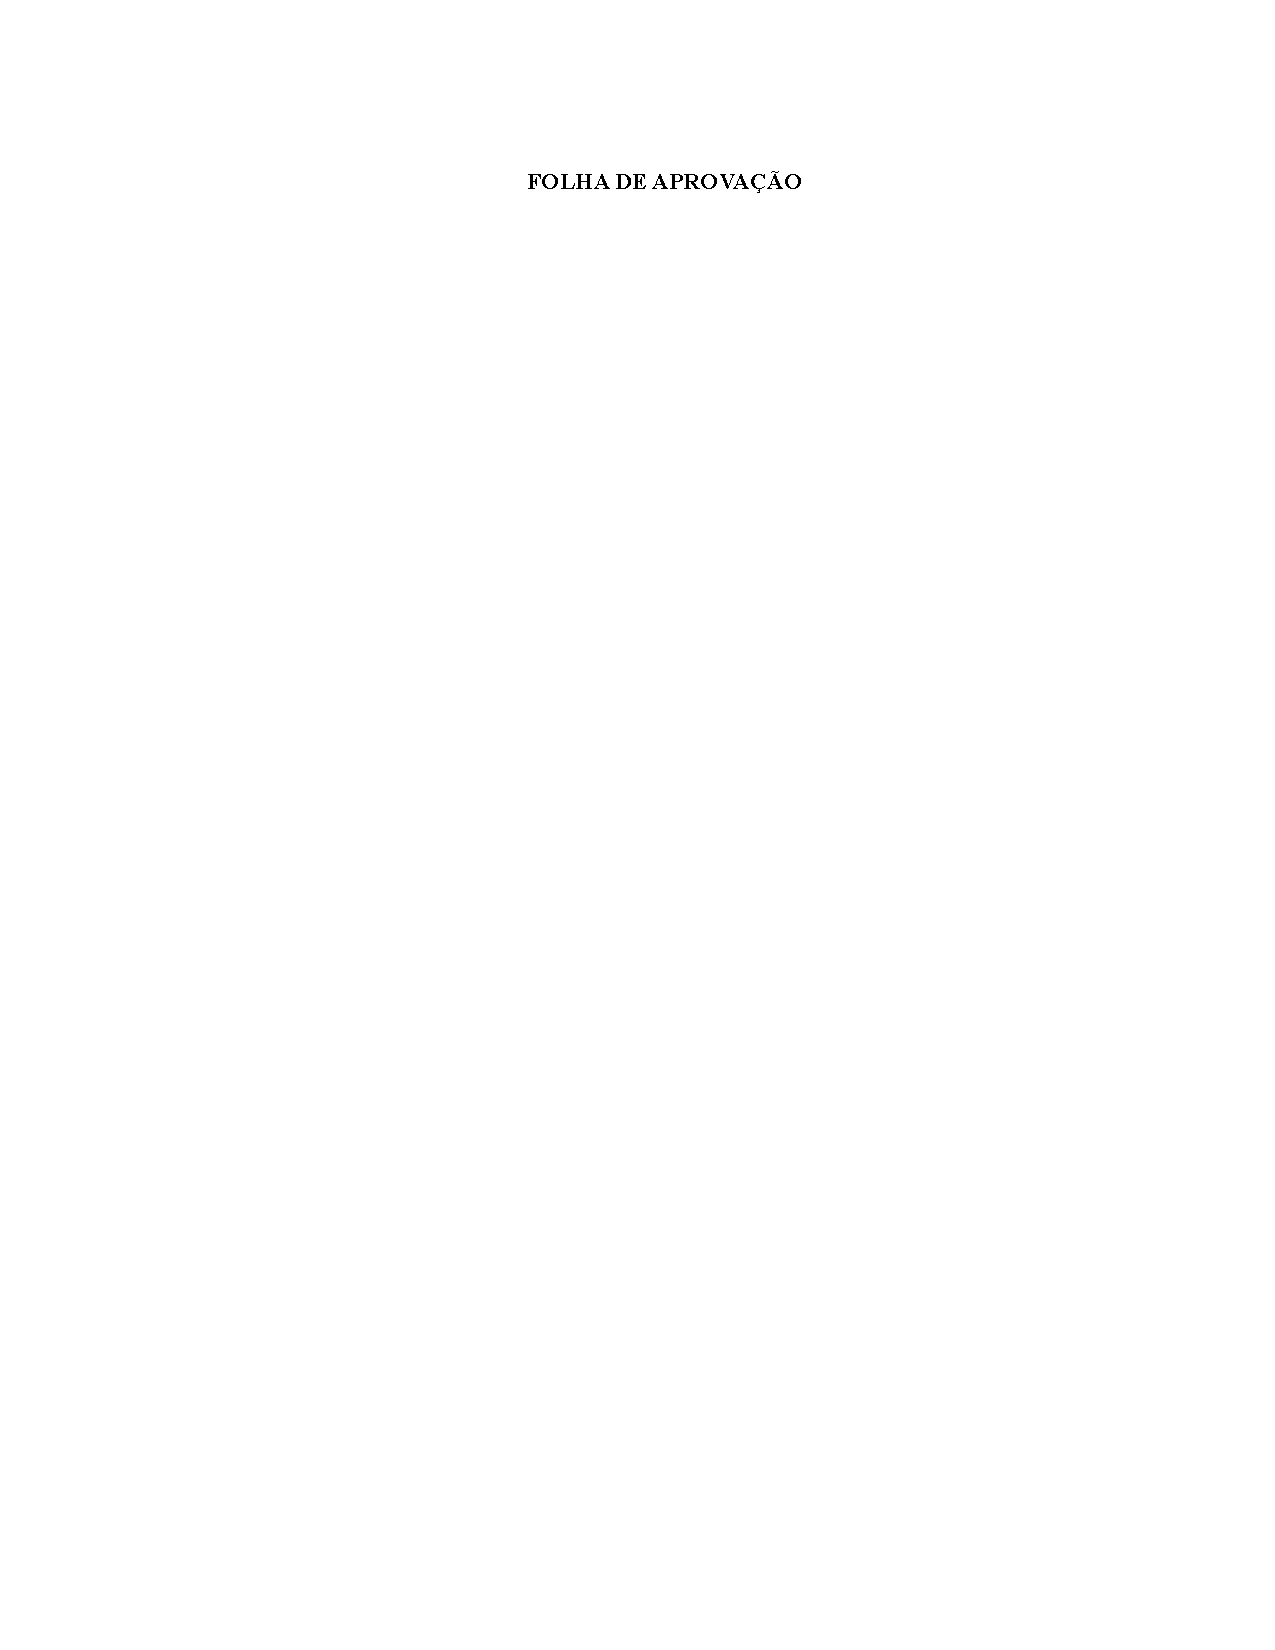
\includepdf[scale=1.0,pages=1]{./PreTexto/folha-aprovacao.pdf} % para adicionar o pdf enviado pelo professor apenas substitua o documento folha-aprovacao.pdf dentro da pasta PreTexto

%% Dedicatória
% %%%% DEDICATÓRIA
%%
%% Texto em que o autor presta homenagem ou dedica seu trabalho.

\begin{dedicatoria}%% Ambiente dedicatoria

Dedico este trabalho à aa, pela referência acadêmica e profissional que sempre foi para mim.

\end{dedicatoria}
%% Comente para remover este item

%% Agradecimentos
% %%%% AGRADECIMENTOS
%%
%% Texto em que o autor faz agradecimentos dirigidos àqueles que contribuíram de maneira relevante à elaboração do trabalho.

\begin{agradecimentos}%% Ambiente agradecimentos

Certamente estes parágrafos não irão atender a todas as pessoas que fizeram parte dessa importante fase de minha vida. Portanto, desde já peço desculpas àquelas que não estão presentes entre essas palavras, mas elas podem estar certas que fazem parte do meu pensamento e de minha gratidão. 

Agradeço ao(a) meu(minha) orientador(a) Prof.(a) Dr.(a) Nome Completo, pela sabedoria com que me guiou nesta trajetória.

Aos meus colegas de sala.

A Secretaria do Curso, pela cooperação.

Gostaria de deixar registrado também, o meu reconhecimento à minha família, pois acredito que sem o apoio deles seria muito difícil vencer esse desafio. 

Enfim, a todos os que por algum motivo contribuíram para a realização desta pesquisa.


Espaço destinado aos agradecimentos (elemento opcional). Folha que contém manifestação de reconhecimento a pessoas e/ou instituições que realmente contribuíram com o(a) autor(a), devendo ser expressos de maneira simples.

Não devem ser incluídas informações que nominem empresas ou instituições não nominadas no trabalho.

Se o aluno recebeu bolsa de fomento à pesquisa, informar o nome completo da agência de fomento. Ex: Capes, CNPq, Fundação Araucária, UTFPR, etc. Incluir o número do projeto após a agência de fomento. Este item deve ser o último.

Atenção: não utilizar este exemplo na versão final. Use a sua criatividade!

\end{agradecimentos}
%% Comente para remover este item

%% Epígrafe
% %%%% EPÍGRAFE
%%
%% Texto em que o autor apresenta uma citação, seguida de indicação de autoria, relacionada com a matéria tratada no corpo do
%% trabalho.

\begin{epigrafe}%% Ambiente epigrafe
Primeira Lei: Um robô não pode ferir um ser humano ou, por omissão, permitir que um ser humano sofra algum mal. Segunda Lei: Um robô deve obedecer as ordens que lhe sejam dadas por seres humanos, exceto nos casos em que tais ordens contrariem a Primeira Lei. Terceira Lei: Um robô deve proteger sua própria existência desde que tal proteção não entre em conflito com a Primeira e Segunda Leis (ASIMOV, Isaac, 1950) - observação: A referência deve ser incluída na lista de referências no final do trabalho.

(elemento opcional)
\end{epigrafe}
%% Comente para remover este item

%% Resumo
%%%% RESUMO
%%
%% Apresentação concisa dos pontos relevantes de um texto, fornecendo uma visão rápida e clara do conteúdo e das conclusões do
%% trabalho.

\begin{resumoutfpr}

O acesso a recursos computacionais de alto desempenho é essencial para a realização de pesquisas acadêmicas e científicas, porém, a aquisição e manutenção de \glspl{desktop} de alto desempenho é um desafio para instituições públicas de ensino superior devido a existência de processos licitatórios complexos e demorados. Por outro lado, universitários advindos de famílias de baixa renda, que não possuem condições financeiras para adquirir um computador pessoal, podem ter dificuldades para realizar atividades acadêmicas dentro e fora da universidade. Sendo assim, o objetivo deste trabalho é desenvolver um sistema de \gls{vdi} capaz de possibilitar que alunos e pesquisadores de instituições de ensino superior acessem \glspl{desktop} virtuais alocados em nuvem pública através de qualquer dispositivo com acesso à internet e com suporte a um navegador web, aprimorando a gestão dos recursos computacionais mais potentes, uma vez que são consumidos como serviço ao invés de serem adquiridos através de processos licitatórios complexos e demorados.


%  %% Ambiente resumoutfpr

%  O resumo deve ressaltar de forma sucinta o conteúdo do trabalho, incluindo justificativa, objetivos,
%  metodologia, resultados e conclusão. Deve ser redigido em um único parágrafo, justificado, contendo
%  de 150 até 500 palavras. Evitar incluir citações, fórmulas, equações e símbolos no resumo.
 
%  A referência no resumo é elemento opcional em trabalhos acadêmicos, sendo que na UTFPR adotamos por
%  não incluí-la nos resumos contidos nos próprios trabalhos. As palavras-chave e as keywords são grafadas
%  em inicial minúscula quando não forem nome próprio ou nome científico e separados por ponto e vírgula.
 
%  % Add a blank line here
 

\end{resumoutfpr}

%% Comente para remover este item

%% Abstract
%%%% ABSTRACT
%%
%% Versão do resumo para idioma de divulgação internacional.

\begin{abstractutfpr} %% Ambiente abstractutfpr

Access to high-performance computing resources is essential for conducting academic and scientific research. However, acquiring and maintaining high-performance \glspl{desktop} is a challenge for public higher education institutions due to the existence of complex and lengthy bidding processes. On the other hand, university students from low-income families, who do not have the financial means to purchase a personal computer, may have difficulties carrying out academic activities both inside and outside the university. Therefore, the objective of this work is to develop a \gls{vdi} system capable of enabling students and researchers from higher education institutions to access virtual \glspl{desktop} allocated in the public cloud through any device with internet access and web browser support, improving the management of the most powerful computing resources, as they are consumed as a service instead of being acquired through complex and lengthy bidding processes.

\end{abstractutfpr}%% Comente para remover este item

%% Lista de algoritmos
%\incluirlistadealgoritmos%% Comente para remover este item

%% Lista de ilustrações
\incluirlistadeilustracoes%% Comente para remover este item

%% Lista de Fotografias
% \incluirlistadefotografias %% Comente para remover este item

%% Lista de Gráficos
% \incluirlistadegraficos %% Comente para remover este item

%% Lista de tabelas
\incluirlistadetabelas%% Comente para remover este item

%% Lista de quadros
% \incluirlistadequadros

%% Listagem de códigos fonte
\incluirlistadecodigosfonte

%% Lista de abreviaturas, siglas e acrônimos
\incluirlistadeacronimos{glossaries}%% Opções: "glossaries" (pacote) ou "file" (arquivo) ou "none" (desabilita)

%% Lista de símbolos
\incluirlistadesimbolos{nomencl}%% Opções: "nomencl" (pacote) ou "file" (arquivo) ou "none" (desabilita)

%% Sumário
\incluirsumario%% Comente para remover este item

%% Formatação de páginas de elementos textuais
\textual%% Não comente esta linha


% \part{Introdução}
%%%% CAPÍTULO 1 - INTRODUÇÃO
%%
%% Deve apresentar uma visão global da pesquisa, incluindo: breve histórico, importância e justificativa da escolha do tema,
%% delimitações do assunto, formulação de hipóteses e objetivos da pesquisa e estrutura do trabalho.

%% Título e rótulo de capítulo (rótulos não devem conter caracteres especiais, acentuados ou cedilha)
\chapter{Introdução}\label{cap:introducao}

Em 1997 o professor de sistemas de informação Ramnath Challappa utilizou o termo Computação em nuvem pela primeira vez para representar um conceito tecnológico que já era utilizado desde os anos 1950. Antes de ganhar o nome mais atual, a tecnologia chegou a ser chamada de \textit{Utility Computing}, fazendo alusão ao acesso compartilhado e de forma simultânea a computadores mainframe, que ocupavam muitas vezes salas completas e custavam caro. \citep{dellcloud}

A computação em nuvem atualmente já aparece como pilar de soluções tecnológicas em situações de escalas variadas. Por um lado, uma grande empresa pode utilizá-la para prover a infraestrutura de grandes aplicações de operação crítica, e por outro lado, um desenvolvedor pode executar cargas de trabalhos em uma instância remota, desativá-la após concluir e pagar apenas pelo tempo de uso do recurso. \citep{taurioncloud}

\textit{VDI} ou Infraestrutura de \textit{desktops} Virtuais é o termo usado para referenciar um ambiente de infraestrutura que hospeda \textit{desktops} virtuais e provê para usuários finais a medida que são requisitados. Tanto ambientes \textit{on premise} quanto em nuvem utilizam a mesma base conceitual de virtualização para tal arquitetura, a grande diferença está na forma em que os recursos são precificados. Em servidores locais, o recurso deve ser comprado previamente, gerenciado e protegido, já em ambientes de nuvem, onde o modelo de responsabilidade compartilhada exime o usuário de responsabilidades de segurança e gerenciamento físicos dos recursos o preço é pago pela utilização dos recursos. \citep{vmwarevdi}

Embora tenham sido feitos progressos utilizando \textit{VDI} em nuvem e a influência dos fatores de qualidade de serviço em sistemas de ensino baseados em \textit{VDI} \citep{qoselearning}, poucos estudos foram realizados com o fim de apresentar uma infraestrutura completa de aplicação que sustente \textit{desktops} virtuais em nuvem pública para utilização em ensino e pesquisa.

O objetivo deste trabalho é propor um formato de infraestrutura de \textit{desktops} virtuais em nuvem pública para sustentar ensino e pesquisa, materializado através de um protótipo de aplicação que garante o acesso à recursos computacionais a partir de qualquer dispositivo com um navegador de internet instalado.

Através da aplicação, os responsáveis pela infraestrutura disponibilizarão templates de imagens\footnote{Templates de images são cópias do sistema operacional com todas as configurações já estabelecidas. Eles facilitam a configuração de um novo \textit{desktop}, reduzindo o tempo até estarem acessíveis para o usuário final} que podem ser usadas. Os professores poderão autorizar e gerenciar quais tipos de imagens, os alunos podem acessar. Por fim os alunos poderão acessar os recursos computacionais de qualquer lugar, dentro ou fora da universidade.

No cenário de uma aula de laboratório onde um conjunto de softwares é necessário para a execução das atividades e os mesmos demandam uma capacidade computacional maior do que os dispositivos físicos dos alunos é capaz de fornecer, ainda sim todos seriam capazes de participar, já que esses dispositivos servem como interface para os recursos computacionais em nuvem.

Em outro cenário, também será possível a um pesquisador acessar recursos computacionais com dados persistidos entre sessões. 

\section{Objetivos}\label{sec:objetivos}

Na seção a seguir, os objetivos que norteiam o desenvolvimento do trabalho serão apresentados na forma de um objetivo principal e objetivos específicos que delimitam as etapas do projeto.

\subsection{Objetivo geral}\label{subsec:objetivoGeral}

O objetivo do trabalho é propor um formato de infraestrutura de \textit{desktops} virtuais em nuvem pública para sustentar ensino e pesquisa.

\subsection{Objetivos específicos}\label{subsec:objetivosEspecificos}

\begin{itemize}
    \item Analisar o desempenho dos protocolos de conexão com \textit{desktops} remotos para definir quais protocolos serão utilizados.

    \item Elaborar um diagrama de arquitetura de aplicação em nuvem.

    \item Desenvolver um protótipo de aplicação baseado no diagrama de arquitetura, com segmentação de acesso por tipo de usuário, onde alunos acessam \textit{desktops} virtuais através de navegadores de internet, professores gerenciam os recursos que os alunos têm acesso e os administradores de sistema disponibilizam templates de máquina que podem ser utilizados dentro da aplicação.

    \item Levantar uma estimativa de custo do protótipo de aplicação construído, levando em consideração aspectos de utilização mensal dos recursos de núvem.
\end{itemize}

\section{Justificativa}\label{sec:justificativa}

Em 2021, o censo de educação superior mostrou que cerca de 3,9 milhões de estudantes ingressaram em instituições de ensino superior e que 77,7\% destes concluíram o ensino médio na rede pública de ensino. \citep{inep2021}
Para aqueles que não possuem computadores portáteis de uso próprio, ainda é um desafio lidar com demandas que exigem o acesso a esse tipo de equipamento.

No contexto da UTFPR, os alunos têm a possibilidade de utilizar os equipamentos em aulas de laboratório ou na biblioteca. Porém a pandemia de COVID-19 evidenciou que essas políticas de acesso ainda não são suficientes para promover o acesso igualitário entre os estudantes.

Esse trabalho apresenta uma proposta de interesse compartilhado. Universidades públicas que dependem de licitação para adquirir equipamentos, otimizarão o uso de seus recursos, uma vez que a solução do trabalho requisita dispositivos com configurações modestas para acesso, abrindo caminho para economia de custos com equipamentos e também para reutilização de computadores com capacidade reduzida, além de promover o acesso facilitado à recursos em nuvem dimensionáveis para pesquisa. E alunos terão a possibilidade de acesso a recursos computacionais através de qualquer dispositivo com acesso à internet e que tenha um navegador web.


\section{Estrutura do trabalho}\label{sec:estruturaTrabalho}

O trabalho está estruturado em três capítulos. O Capítulo 1 apresenta o assunto do trabalho, bem como o tema e os objetivos da produção. O Capítulo 2 detalha os conceitos utilizados para a concepção do projeto, o estado da arte e mostra outros trabalhos e pesquisas que já foram publicados e que estão relacionados com o tema do atual trabalho. Por fim, o Capítulo 3 descreve quais materiais e métodos serão empregados para o cumprimento dos objetivos propostos, bem como o cronograma de atividades a serem realizadas.
%%%% CAPÍTULO 2 - REVISÃO DA LITERATURA (OU REVISÃO BIBLIOGRÁFICA, ESTADO DA ARTE, ESTADO DO CONHECIMENTO)
%%
%% O autor deve registrar seu conhecimento sobre a literatura básica do assunto, discutindo e comentando a informação já publicada.
%% A revisão deve ser apresentada, preferencialmente, em ordem cronológica e por blocos de assunto, procurando mostrar a evolução do tema.
%% Título e rótulo de capítulo (rótulos não devem conter caracteres especiais, acentuados ou cedilha)
\chapter{revis\~ao Da Literatura}
\label{cap:revisaoDaLiteratura}

Esse capítulo apresenta os principais conceitos envolvidos na construção desse trabalho, a fim de contextualizar as bases teóricas utilizadas como referência para o desenvolvimento. O capítulo está organizado em duas seções, na primeira com aspectos do referencial teórico e na segunda com a apresentação de trabalhos relacionados.

\section{Computa\c{c}\~ao em Nuvem}
\label{sec:computacaoEmNuvem}

A computação em nuvem é um termo que se refere ao modelo de de entrega de recursos computacionais, baseado em uma grande rede de servidores físicos ou virtuais. Recursos como capacidade computacional ou capacidade de armazenamento são virtualizados em \textit{data centers} e consumidos sob demanda remotamente. Segundo \citet{taurioncloud}, as principais características são:

\begin{itemize}
    \item A computação em nuvem transmite uma sensação de disponibilidade infinita de recursos.

    \item Com esse tipo de modelo de serviços computacionais, não é necessário adquirir equipamentos físicos para poder utilizá-los. Os mesmo são acessáveis como serviços.

    \item Os recursos podem ser utilizados na proporção que são necessários para determinado cenário, podendo redimensionar a capacidade computacional de forma dinâmica.

    \item O modelo de cobrança em ambientes de nuvem é baseado na quantidade de uso dos recursos.
\end{itemize}

Os serviços de computação em nuvem podem ser classificados de acordo com o modelo de entrega de recursos, bem como o nível de responsabilidade que o usuário tem sobre a infraestrutura que suporta os serviços. Entre os modelos de entrega de recursos, os mais comuns são: \textit{Software as a Service} (SaaS), \textit{Platform as a Service} (PaaS) e \textit{Infrastructure as a Service} (IaaS). \citep{cloudcomputingcambridge}

A \autoref{fig:serviceDeliveryModels} apresenta um diagrama que ilustra a hierarquia de responsabilidades entre os modelos de entrega de recursos. O diagrama mostra que o \textit{SaaS} é o modelo que demanda menos responsabilidade do cliente, mas também entrega mais valor e abstração. O \textit{IaaS} é o modelo que demanda mais responsabilidade do cliente, mas também entrega mais controle sobre a infraestrutura. A \autoref{fig:deliveryModelResponsabilities} apresenta um diagrama que ilustra as responsabilidades de cada modelo de entrega de recursos. \citep{cloudcomputingcambridge}

\begin{figure}[H]
\captionsetup{width=.7\textwidth}%% Largura da legenda
\caption{Modelo de entrega de conteúdo em computação em nuvem}
\label{fig:serviceDeliveryModels}
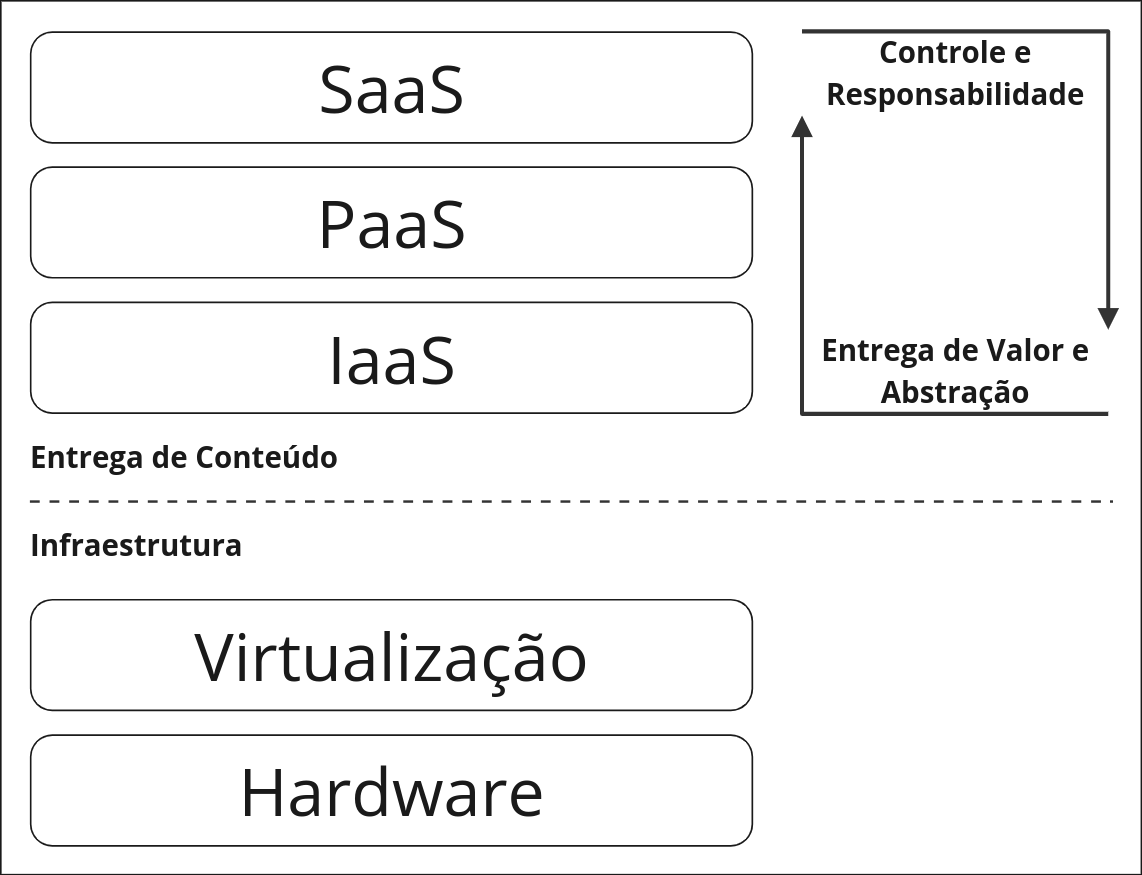
\includegraphics[width=.7\textwidth]{capitulos/1-revisao-da-literatura/files/deliovery-model.png}
\fonte{Adaptado de \citet{cloudcomputingcambridge}}
\end{figure}

\begin{figure}[H]
\captionsetup{width=.7\textwidth}%% Largura da legenda
\caption{Responsabilidades nos modelos de entrega de conteúdo em computação em nuvem}
\label{fig:deliveryModelResponsabilities}
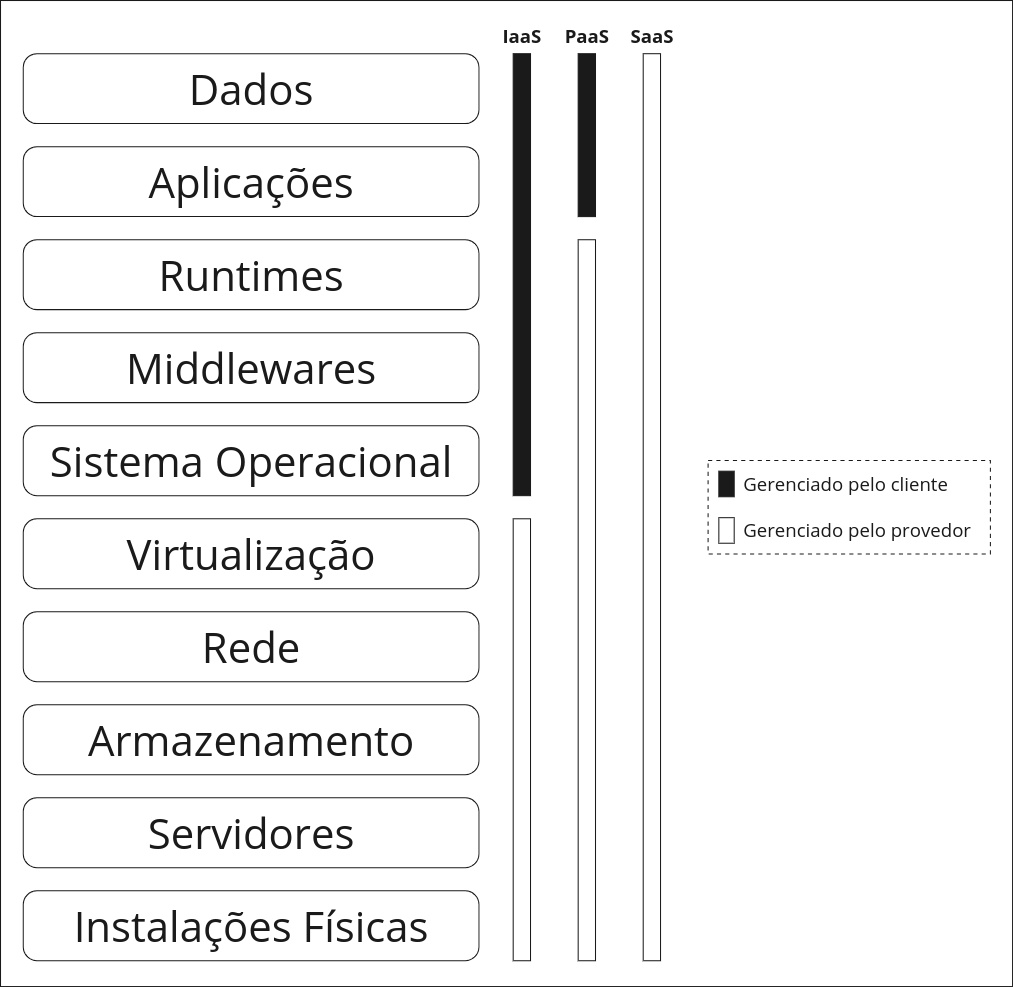
\includegraphics[width=.7\textwidth]{capitulos/1-revisao-da-literatura/files/delivery-model-2.png}
\fonte{Adaptado de \citet{cloudcomputingcambridge}}
\end{figure}

No modelo de entrega \textit{SaaS} o cliente acessa diretamente uma aplicação e o provedor é inteiramente responsável pelo gerenciamento e configuração da infraestrutura que o suporta. No \textit{PaaS} o cliente é capaz de executar e gerenciar aplicações sem a necessidade de se preocupar com a infraestrutura que suporta as aplicações e no \textit{IaaS} o cliente tem controle total sobre a todos os aspectos que compõem a representação virtualizada da infraestrutura. \citep{cloudcomputingcambridge}

Um exemplo de serviço gerenciável é o \textit{Elastic Beanstalk}, que é categorizado como \textit{Paas}. Com ele é possível executar aplicações sem a necessidade direta de configurar a maior parte dos serviços de infraestrutura disponíveis. O desenvolvedor precisa se preocupar somente com o código da aplicação.

Esse tipo de serviço é útil para soluções comuns como \textit{APIs} que necessitam na maioria dos casos dos mesmos componentes de infraestrutura como: Um servidor de aplicação, configuração de rede, balanceador de carga, banco de dados e um local para armazenamento de objetos.

A \textit{AWS} opera seus recursos a partir de um modelo de responsabilidade compartilhada que visa reduzir a responsabilidade operacional dos clientes sobre recursos. \citep{awssharedresponsibilitymodel} E seguindo o modelo, a sua responsabilidade é garantir a segurança \textbf{DA} nuvem. Isso significa que a provedora deve proteger todos os aspectos de infraestrutura que executa os serviços disponibilizados.

Para o cliente, a responsabilidade é de garantir a segurança \textbf{NA} nuvem, levando em consideração todas as boas praticas de desenvolvimento para que os recursos sejam utilizados de maneira responsável e segura.

\section{Virtualização}
\label{sec:virtualization}

A virtualização é uma técnica que permite a representação de recursos computacionais físicos através de uma camada de software que permite a utilização de recursos de maneira customizada e independente para cada necessidade, diferente da abordagem tradicional onde os recursos físicos são acessados diretamente. \citep{cloudcomputingcambridge}

Qualquer tipo de recurso computacional pode ser virtualizado, como processadores, memória, armazenamento e redes. Partindo de um modelo estrutural onde os recursos físicos são interligados e compartilhados, a virtualização permite a criação de ambientes isolados e independentes, onde cada recurso é acessado de maneira exclusiva. Ainda, a técnica de virtualização permite que um recurso físico seja representado através de múltiplos recursos virtuais, como mostra a \autoref{fig:virtualization}, viabilizando assim o modelo de Computação em Nuvem. \citep{cloudcomputingcambridge}

\begin{figure}[H]
\captionsetup{width=.7\textwidth}%% Largura da legenda
\caption{Transformação de recursos físicos em recursos virtuais através da virtualização}
\label{fig:virtualization}
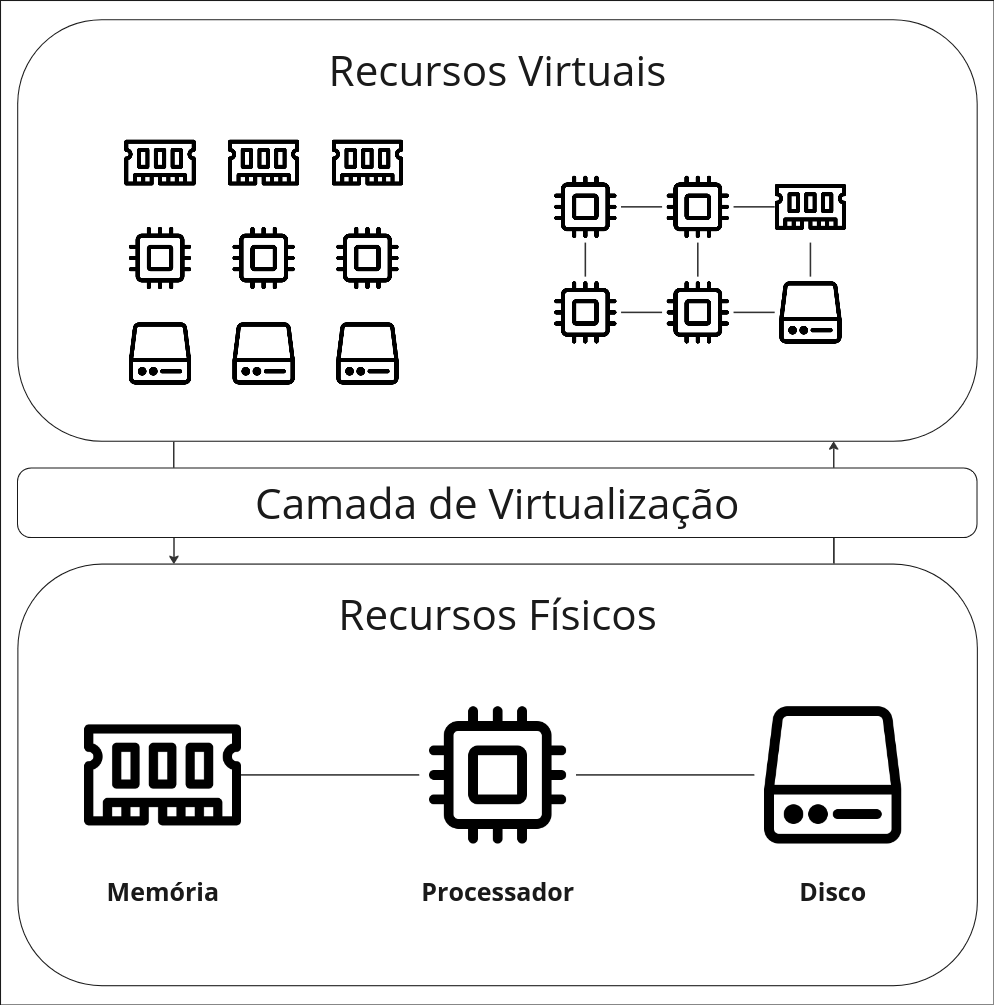
\includegraphics[width=.7\textwidth]{capitulos/1-revisao-da-literatura/files/virtualization-layers.png}
\fonte{Adaptado de \citet{cloudcomputingcambridge}}
\end{figure}

% Infraestrutura virtual de \textit{desktops} é uma técnica que permite o acesso a \textit{desktops} virtualizados através de uma conexão de rede. O conceito engloba os aspectos de hardware, software e infraestrutura necessários para o acesso remoto. \citep{techopediavdi}

% Em um ambiente de \textit{VDI}, todas as configurações de sistema operacional e preferências ficam armazenadas no \textit{host}. Para o usuário, a experiência de acesso é similar ao uso de um computador local.

% A maneira que os \textit{desktops}  são distribuídos entre os usuários depende da implementação do serviço e costuma seguir um dos dois padrões a seguir: \citep{vdiieexplore}

% \begin{enumerate}
%     \item Implementação dedicada: Nela, o \textit{desktop} é alocado especificamente para um usuário, e caso o ambiente não seja volátil, não é necessário a existência de um mecanismo de backup para as configurações salvas.

%     \item Implementação em pool: Nesse padrão, quando o usuário acessa um \textit{desktop}, o servidor cria a conexão com o próxima instância disponível no sistema. Isso significa que a cada acesso, as configurações serão reiniciadas para o padrão de inicialização do sistema. É comum nesses casos que o servidor mantenha um número mínimo de instâncias previamente inicializadas para diminuir o tempo de conexão.
% \end{enumerate}



% Arquitetura hexagonal
\section{Arquitetura Hexagonal}
\label{sec:arquiteturaHexagonal}

Arquitetura hexagonal é um padrão de arquitetura de software proposto por Alistair Cockburn em 2005, que ajuda a solucionar problemas de testabilidade e acoplamento de componentes em sistemas de software. Quando um software é projetado, muitas vezes é difícil projetar componentes genéricos o suficiente para que não dependam de um determinado \textit{framework} ou tecnologia. Isso é problemático porque a manutenção do software se torna mais difícil e a escolha de novas tecnologias pode ser limitada, além de tornar o processo de testes complexo e custoso. Para resolver esses problemas, a arquitetura hexagonal propõe uma abordagem onde o núcleo da aplicação é responsável por orquestrar todas as operações de entrada e saída de dados através de adaptadores. \citep{cockburn2017}.

Como pode ser visto na \autoref{fig:hexagonalArchitecture}, o padrão é representado por um hexágono com a aplicação no centro. As arestas do hexágono delimitam as fronteiras dos casos de uso da aplicação e também representam os \textit{Ports}, que são as interfaces as interfaces de comunicação entre a camada de aplicação e a camada de interfaces \citep{cockburn2017}.

\begin{figure}[H]
% \captionsetup{width=.7\textwidth}%% Largura da legenda
\caption{Arquitetura hexagonal}
\label{fig:hexagonalArchitecture}
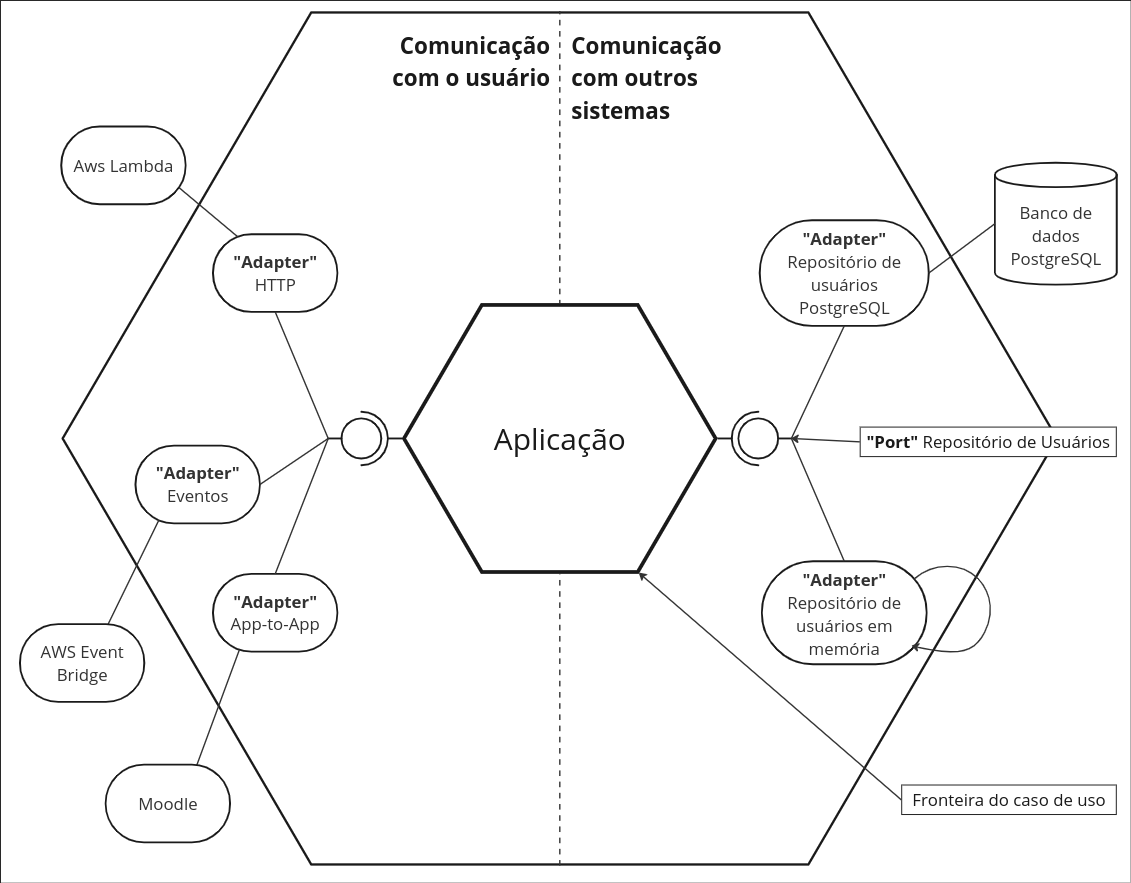
\includegraphics[width=\textwidth]{capitulos/1-revisao-da-literatura/files/hexagonal.png}
\fonte{Adaptado de \citet{cockburn2017} e \citet{awsHexagonalArchitecture}}
\end{figure}

Os adapter são classes que implementam as interfaces definidas pelos \textit{Ports}, neles a lógica de comunicação com quaisquer componente externo é implementada. Dessa forma, a aplicação não precisa saber de detalhes técnicos de cada componente externo, como por exemplo, a forma de comunicação com um banco de dados ou a forma de comunicação com um serviço de mensageria. \citep{cockburn2017}.

No momento da criação de testes unitários para os casos de uso da aplicação, os \textit{Adapters} que utilizam comunicação externa são substituidos por outros \textit{Adapters} que simulam a comunicação externa. Isso permite que os testes sejam executados de maneira independente e sem a necessidade de outros serviços externos. Na imagem \autoref{fig:hexagonalArchitecture}, existe um exemplo de \textit{Port} para armazenamento de informações de usuários, bem como dois \textit{Adapters} que implementam a interface do \textit{Port}. Um dos \textit{Adapters} é responsável por armazenar as informações em um banco de dados e o outro é responsável por armazenar as informações em memória. Ambos são utilizados dentro do ciclo de desenvolvimento, mas em momentos diferentes, sendo um para testes e outro para a execução real da aplicação.

No desenvolvimento prático utilizando \textit{Ports and Adapters}, padrões como o \textit{Domain Driven Design} o \textit{SOLID} e a injeção de dependências são comumente utilizados em conjunto \citep{cockburn2017}.





% A arquitetura hexagonal é um padrão de arquitetura de software proposto por Alistair Cockburn em 2005, com o objetivos de criar \textit{softwares} desacoplados onde os componentes possam ser testados de maneira independente. Além disso, o padrão ajuda a evitar que a implementação das regras de negócio fiquem acopladas a um determinado \textit{framework} ou tecnologia. \citep{awsHexagonalArchitecture}.


% Nesse padrão, a aplicação é representada por um exágono, onde cada lado representa uma porta de entrada ou saída de dados. As portas de entrada são responsáveis por receber os dados de entrada e as portas de saída são responsáveis por enviar os dados de saída. O núcleo da aplicação é responsável por orquestrar a comunicação entre as portas de entrada e saída. \citep{awsHexagonalArchitecture}.



\section{Trabalhos Relacionados}
\label{sec:trabalhosRelacionados}

O trabalho desenvolvido por \citet{qoselearning} realiza uma análise quantitativa do impacto de
parâmetros de conexão de rede em ambientes de ensino remoto sustentados por uma estrutura de \gls{vdi}.
A análise é feita a partir de um experimento com o objetivo de clarificar a relação entre a qualidade de
conexão com a internet e a usabilidade de sistemas de ensino remoto.

O resultado do experimento mostrou que é possível realizar atividades como escrita, desenhos e
consumo de mídias, sem grandes prejuízos para a usabilidade, mas é necessário que a conexão com a
internet tenha qualidade. Outro ponto importante é que fora atividades de visualização de vídeos, a
largura de banda não é um fator de grande consumo nesses tipos de ambientes.

Outro trabalho de grande relevância para essa produção, desenvolvido por \citet{edufirestick},
apresenta um sistema de \gls{vdi} para educação remota utilizando as mesmas tecnologias propostas
no presente trabalho. 

A proposta da produção é de criar uma \gls{vdi} de baixo custo com \glspl{ec2SpotInstance} da
\gls{aws} e com o \gls{guacamole} para gerenciamento das conexões, e permitindo o acesso de
qualquer dispositivo com um navegador de internet, até mesmo através televisões com acesso à internet,
como apresentado no trabalho.

A solução proposta por \citet{edufirestick} aborda um cenário de aula de laboratório, onde um
professor pode agendar um evento de criação das máquinas virtuais para os alunos e no horário da
aula, todos poderiam acessar o recurso reservado para a aula.

Em termos de custos operacionais, o trabalho apresenta uma estimativa de custo por usuário de
USD\$ 0.87 mensais com a utilização dos seguintes parâmetros:

\begin{itemize}
    \item Tempo de conexão diária: 18 horas
    \item Categoria da instância: t3.micro
    \item Sistema operacional: \textit{Microsoft Windows Server 2019}
    \item Memória: 4 GB de \gls{ram}
    \item Espaço em disco: 90 GB
    \item Região: São Paulo
\end{itemize}

Em termos de preço pela transferência de dados, o trabalho relata um custo de USD\$ 0.06 por hora em
picos onde o uso de banda chaga a 2 MB/s. O custo dos outros serviços que suportam a infraestrutura,
foi estimado em USD\$ 200.00 mensais.

O trabalho feito por \citet{edufirestick} apresenta um panorama muito promissor e consoante aos
objetivos do presente trabalho, demostrando que é possível executar a solução em um cenário de
laboratório. Mas ainda não apresenta resultados referentes ao gerenciamento de \glspl{desktop} que
tenham os dados persistidos, para outros cenários de uso, como o de pesquisa por exemplo.
%%%% CAPÍTULO 3 - MATERIAL E MÉTODOS (PODE SER OUTRO TÍTULO DE ACORDO COM O TRABALHO REALIZADO)

\chapter{Metodologia}\label{cap:metodologia}

% A ênfase deste capítulo está em reportar o que e como será feito para alcançar o objetivo do trabalho. Este capítulo pode ser subdividido, inicialmente, em duas seções, sendo uma para os materiais e outra para os métodos.

Este capítulo apresenta o plano de trabalho a ser seguido para que os objetivos citados
anteriormente sejam alcançados. Primeiramente, ferramentas e tecnologias utilizadas serão discutidas seguidas dos métodos a serem empregados para que os objetivos sejam atingidos.

\section{Materiais}\label{sec:materiais}

O objetivo do trabalho é apresentar um modelo de arquitetura voltado para nuvem, e para tal, algumas ferramentas e tecnologias foram escolhidas para a construção da solução.

\subsection{Amazon Web Services}\label{subsec:amazonWebServices}

Popularmente conhecida pela sigla \textit{AWS}, a empresa subsidiária da Amazon detêm a maior fatia de mercado do segmento de computação em nuvem. A \textit{AWS} foi escolhida como provedor de serviços de nuvem porque disponibiliza uma gama de serviços que possibilitam a execução do trabalho.

A princípio o projeto contará com os seguintes recursos oferecidos pela \citet{awsconceitosbasicos}: 

\begin{itemize}

    \item \textbf{\textit{Elastic Cloud Computing (EC2)}}: São instâncias virtualizadas que serão utilizadas como desktop virtual para o usuário final.
    
    \item \textbf{\textit{Lambda}}: São funções \textit{serverless}\footnote{funções serverless fazem uma abstração a nível de aplicação para que o desenvolvedor consiga executar literalmente funções de código em um ambiente de nuvem sem a necessidade de configurar uma aplicação ou o servidor que a hospeda} que executarão parte da lógica envolvida na aplicação. Essas funções são executadas a medida que são requisitadas, e são desativadas com inatividade.
    
    \item \textbf{\textit{Simple Storage Service (S3)}}: É um serviço de armazenamento de objetos que será utilizado para guardar dados estáticos, como arquivos de texto, fotos ou vídeos.
    
    \item \textbf{\textit{Event Bridge}}: É um serviço que possibilita a comunicação entre recursos através de eventos. Com ele é possível publicar e consumir eventos com informações customizadas.
    
    \item \textbf{\textit{Fargate, Elastic Container Service (ECS) e Elastic Container Registry (ECR)}}: Os serviços são altamente relacionados e servem para orquestrar e executar aplicações baseadas em containers. De forma simples, o \textit{ECR} armazena as imagens de containers, o \textit{Fargate} é o ambiente de execução e o \textit{ECS} atua como orquestrador entre os dois outros serviços. Eles serão responsáveis por executar o serviço que conecta os usuários aos seus respectivos \textit{desktops} virtuais.
    
    \item \textbf{\textit{Aurora Serverless}}: É um serviço de banco de dados relacional serverless que será utilizado para armazenar todas as informações derivadas de regras de negócio.

    \item \textbf{\textit{Cloud Development Kit (CDK)}}: É um \textit{framework}\footnote{Um framework é um conjunto de bibliotecas que auxiliam no desenvolvimento de aplicações} utilizado para a definição da infraestrutura de forma programática. Ao contrário de configurar os recursos de nuvem manualmente, com o \textit{CDK} é possível descrever como código, quais são os recursos a serem alocados e suas comunicações. Ele é imprescindível no trabalho, já que possibilita a replicação do modelo de arquitetura.
    
\end{itemize}

Todos os serviços acima certamente serão utilizados, porém existem outros serviços que não foram listados porque não há argumentos suficientes nessa etapa do projeto para listá-los.

A execução do trabalho conta também com um apoio da \textit{AWS} em forma de créditos a serem utilizados na plataforma e assistência técnica de um intermediário.

\subsection{Apache Guacamole}\label{subsec:apacheGuacamole}

O Apache Guacamole é uma aplicação gratuita de código aberto definido como: \textit{clientless remote desktop gateway}. \citep{apacheguacamole} Com uma tradução livre, seria um portão para acesso a \textit{desktops} remotos sem cliente.

O termo \textit{clientless} remete ao fato da aplicação ser agnóstica quando ao cliente que a consome. Isso significa que existe um protocolo de conexão bem definido e documentado, que pode ser reproduzido em qualquer linguagem de programação. 

No contexto desse trabalho o cliente da aplicação implementará o protocolo do guacamole para se comunicar com o servidor, que por sua vez efetuará a conexão do usuário.


\subsection{Node.js}\label{subsec:nodeJs}

O Node.js é um ambiente de execução de \textit{javascript} baseado em eventos assíncronos otimizado para a criação de aplicações de rede escaláveis. Ele será utilizado dentro das funções \textit{serverless} para executar partes das lógicas de negócio. \citep{nodejs}

Ele foi escolhido por ter hoje uma das maiores comunidades de desenvolvedores ativos, além de fornecer artefatos para a implementação das lógicas a serem desenvolvidas.

\subsection{Next.js}\label{subsec:nextJs}

O Next.js é um \textit{framework} de código aberto para o desenvolvimento de aplicações web. Com ele é possível executar renderização de elementos de tela no servidor e também geração de páginas estáticas. \citep{nextjs}

Ele foi escolhido para esse trabalho para a criação do sistema web, intermediando a conexão com os servidores da infraestrutura. Toda a lógica de autenticação, visualização dos componentes disponíveis e gerenciamento dos recursos, exceto criação dos templates de imagem de máquina, serão implementados nesta aplicação web.

% Materiais são as ferramentas, as tecnologias, os ambientes de desenvolvimento e outros que são utilizados para realizar as atividades desde a definição dos requisitos à implantação do sistema. Exemplos de materiais: linguagens de programação e de modelagem, banco de dados e seus gerenciadores, editores para análise e modelagem, ambiente e plataforma de desenvolvimento.

% Cada um dos materiais pode ter uma subseção própria ou serem descritos em uma mesma seção. De qualquer forma, essa seção não precisa ser muito extensa, deve abranger apenas um conhecimento básico sobre cada um dos materiais e o que é mais relevante ou utilizado para o trabalho proposto. De maneira geral, não há necessidade de incluir informações históricas sobre os materiais. Centrar-se nos conceitos e particularidades mais relevantes para o trabalho. Exceto se necessário para o entendimento do objeto do trabalho ou considerado relevante para o tipo de pesquisa.

\section{Métodos}\label{sec:metodo}

Inicialmente, um estudo será realizado para analisar a performance dos protocolos de conexão com \textit{desktops} remotos já presentes no Apache Guacamole, sendo eles \textit{SSH}, \textit{VNC} e \textit{RDP}. Como os protocolos estão em uma camada mais abstrata da solução, a viabilidade de implementação de um outro protocolo ainda não integrado com o Guacamole será avaliada e implementada, se possível. Caso contrário será listada como aprimoramento do trabalho atual.

Durante o estudo diversos cenários de conexão serão testados, visando cobrir casos de uso onde softwares que demandam maior capacidade de processamento de vídeo são utilizados. Como resultado, são esperados parâmetros para nortear o dimensionamento dos recursos computacionais empregados na solução.

Em seguida, um diagrama de infraestrutura será construído com o apoio de uma equipe especializada da \textit{AWS}, que ajudará na idealização dos componentes e identificação de pontos a serem otimizados. Como resultado, espera-se uma base conceitual da infraestrutura para nortear o desenvolvimento.

A partir desse momento, o protótipo da aplicação será construído a partir das seguintes etapas:

\begin{enumerate}
    \item Configuração das bases de código com versionamento, suporte a documentação, integração e entrega contínuas.
    \item Configuração da conta na \textit{AWS} com ativação dos créditos cedidos pela empresa.
    \item Configuração dos componentes de servidor do Apache Guacamole.
    \item Desenvolvimento das lógicas de negócio com funções \textit{serverless}.
    \item Desenvolvimento dos componentes da arquitetura como código.
    \item Desenvolvimento da aplicação web.
\end{enumerate}

Com o protótipo construído, algumas métricas de custo serão avaliadas para que uma estimativa de custo de aplicação seja descrita, levando em consideração parâmetros de utilização coerentes com o cenário atual da UTFPR. Como resultado, é de interesse saber se a implementação do projeto é viável economicamente.

Por fim, o projeto será documentado e apresentado à universidade em forma de proposta de implementação.

\section{Requisitos Funcionais}\label{sec:requisitosFuncionais}

O desenvolvimento do protótipo será realizado com base em requisitos funcionais. Estes que por sua vez fundamentam uma base aceitável de funcionalidades e casos de uso que fazem sentido para a utilização do projeto como solução de software. São eles:

\begin{itemize}
    \item \textbf{RF-001}: O software deverá permitir o login de usuários através das credenciais institucionais.

    \item \textbf{RF-002}: O software deverá distinguir os usuários com base em seu papel dentro da instituição. (Aluno, Professor, Administrador do Sistema)

    \item \textbf{RF-003}: O software deverá permitir que o usuário (aluno e professor) liste os \textit{desktops} que tem acesso.

    \item \textbf{RF-004}: O software deverá permitir que o usuário (aluno e professor) inicie uma sessão com um \textit{desktop} que tenha acesso.
    
    \item \textbf{RF-005}: O software deverá permitir que o usuário (aluno e professor) finalize a sessão com um \textit{desktop} que tenha acesso.
    
    \item \textbf{RF-006}: O software deverá permitir que o usuário (aluno e professor) mantenha a sessão ativa com um \textit{desktop} mesmo que o software seja fechado.
    
    \item \textbf{RF-007}: O software deverá permitir que o usuário (aluno e professor) exclua um \textit{desktop} que tenha acesso.

    \item \textbf{RF-008}: O software deverá permitir que o usuário (aluno e professor) crie um novo \textit{desktop} a menos que tenha atingido o máximo de sua permissão.
    
    \item \textbf{RF-009}: O software deverá permitir que o usuário professor altere os limites de utilização de um usuário aluno.

    \item \textbf{RF-010}: O software deverá estabelecer a conexão com o \textit{desktop} utilizando uma conexão criptografada via \textit{SSL}.

    \item \textbf{RF-011}: O software deverá permitir que o usuário (professor) liste os alunos que utilizam o software.

    \item \textbf{RF-012}: O software deverá encerrar \textit{desktops} inativos que não foram previamente configurados para permanecer ininterruptos.
    
    \item \textbf{RF-013}: O software deverá coletar métricas de utilização dos \textit{desktops}.
    
    \item \textbf{RF-014}: O software deverá permitir ao usuário a visualização das métricas coletadas, respeitando sua política de acesso.
    
    \item \textbf{RF-015}: O software deverá emitir alertas via e-mail do tempo de utilização em casos onde o \textit{dekstop} não é programado para desligar automaticamente.
    
    \item \textbf{RF-016}: O software deverá permitir que o usuário (administrador) crie templates de imagem de máquina.
    
    \item \textbf{RF-017}: O software deverá permitir que o usuário (administrador) delete templates de imagem de máquina.

    \item \textbf{RF-018}: O software deverá registrar todas as ações auditáveis realizadas dentro do software.

    \item  \textbf{RF-019}: O software deverá permitir que o usuário (professor e administrador) liste todas as ações auditáveis.
    
\end{itemize}

\section{Requisitos Não Funcionais}\label{sec:requisitosFuncionais}

Além dos requisitos funcionais, a construção do protótipo levará em conta os seguintes requisitos não funcionais:

\begin{itemize}
    \item \textbf{RNF-001}: O software deverá permitir o acesso através de um navegador web.

    \item \textbf{RNF-002}: O software deverá ser construído de maneira replicável, sem a necessidade de configuração manual do ambiente de nuvem.

    \item \textbf{RNF-003}: O software deverá ser acessível, seguindo as boas práticas de desenvolvimento para a plataforma.
\end{itemize}


% Os métodos definem, de certa maneira, um plano geral do trabalho, com as principais atividades realizadas durante seu processo de desenvolvimento. São apenas as atividades, o que será feito e o que se espera obter com as mesmas. O que é obtido com a realização dessas atividades está no \autoref{cap:resultados}. 

% Os métodos são, basicamente, uma sequência de atividades realizadas para definir o sistema, modelar o problema e a solução, implementar a solução, testar e implantar essa solução. Essas atividades devem enfatizar a forma de uso dos materiais de acordo com o referencial teórico e como foi procedido no sentido de alcançar os objetivos do trabalho.
% Os métodos incluem os procedimentos utilizados para se alcançar o objetivo do trabalho. Assim, ele abrange o ciclo de vida do sistema, da identificação do problema à implantação da solução. A identificação pode incluir a definição dos requisitos por parte do usuário e/ou cliente definindo a proposta do sistema. A implantação pode incluir a forma de gerar os instaladores, os recursos e forma de instalação do sistema, a forma de manutenção e de descontinuidade do sistema.

% A definição das atividades, passos, ou procedimentos que compõem os métodos podem (ou mesmo deve) estarem baseados em autores. Esses autores, normalmente, estão relacionados à engenharia de software.

% O tempo verbal a ser utilizado na descrição dos métodos é o passado, considerando que trata-se de métodos que foram aplicados para a obtenção dos resultados a serem apresentados.

%%%% CAPÍTULO 4 - RESULTADOS E DISCUSSÃO

\chapter{Resultados}
\label{cap:resultados}

Este capítulo apresenta aspectos da implementação do sistema proposto, bem como as discussões acerca
das métricas obtidas durante os testes realizados.

O capítulo está divido em sete seções.
A \autoref{sec:escopoSistema} busca considerar aspectos técnicos e conceituais do sistema afim de delimitar o escopo do sistema.
Na \autoref{sec:modelagemSistema} os diagramas e processos de modelagem do sistema são apresentados
seguindo as definições formais apresentadas no \autoref{cap:materiaisemetodos}.
A \autoref{sec:apresentacaoSistema} apresenta o sistema do ponto de vista do usuário, focando nas funcionalidades e interações com o sistema,
já a \autoref{sec:implementacaoSistema} foca em nos aspectos técnicos mais relevantes na implementação do sistema.
A \autoref{sec:implantacaoSistema} apresenta os cenários de implantação do sistema, trazendo perspectivas de uso e capacidade de escala.
Na \autoref{sec:discussoes} aspectos relevantes dos resultados de testes e discussões são apresentados.
Por fim, os trabalhos e produções tecnológicas que buscam resolver problemas semelhantes ao proposto neste trabalho são apresentados na \autoref{sec:trabalhosRelacionados}.

% Este capítulo apresenta o que foi obtido como resultado do trabalho, que, em princípio, é o sistema desenvolvido. Se não for um sistema, como, por exemplo, uma solução na área de redes, neste capítulo é reportada a solução proposta. Neste caso, a divisão do capítulo em seções é realizada, se necessária, de acordo com o trabalho.

% O capítulo pode conter seções de acordo com o tipo de sistema e a necessidade de documentação mais extensa de determinados aspectos. Caso o trabalho se refira à comparação entre tecnologias ou dados obtidos como resultados do uso do sistema, além da descrição do sistema, há os dados obtidos com os testes e a discussão desses dados. Nesse caso haverá uma seção para os dados obtidos desses testes e as discussões.

\section{Escopo do sistema}
\label{sec:escopoSistema}

O sistema \textit{Virtual Lab} deve possibilidar a criação e gerenciamento de instâncias de máquinas virtuais para uso em laboratórios remotos de ensino e pesquisa.
O acesso deve ser feito por meio de um navegador de internet, permitindo a utilização de qualquer dispositivo com um navagador de internet com acesso à rede.

O sistema deve acomodar dois tipos de usuários: usuários comuns e administradores.
Os usuários comuns devem ter permissão de criar instâncias de máquinas virtuais com base em templates pré-definidos, gerenciar suas próprias instâncias, bem como o conteúdo instalado nas mesmas.
Os administradores devem ter as mesmas permissões dos usuários comuns, além de gerenciar os templates de instância, controlar o acesso dos usuários comuns ao sistema e aos recursos de hardware.

O sistema deve permitir o acesso aos usuários através de autenticação por meio de usuário e senha, bem como através de um provedor de identidade externo, caso o ambiente de uso do sistema já possua um provedor de identidade.

Inicialmente, um usuário administrador deve criar os templates de instância indicando o sistema operacional e a quantidade de armazenamento disponível.
Os usuários comuns devem então criar instâncias com base nesses templates, escolhendo entre os tipos de hardware permitidos.

Ao ser criada, a instância deve passar por um processo de configuração inicial para garantir que o sistema operacional esteja pronto para uso, e então ser disponibilizada para o usuário, que poderá acessá-la atráves da página de conexões do sistema. As instâncias devem ser encerradas automaticamente após um período de inatividade.

\section{Modelagem do sistema}
\label{sec:modelagemSistema}

TODO

% A modelagem do sistema inclui os diagramas e as descrições textuais para representar o problema e a solução.

% Sendo assim, primeiramente esse item deve apresentar diagramas utilizados para a modelagem de negócios (ex. diagramas de atividade e estado), se esses tenham sido necessários.
% Em seguida esse item deve conter a descrição dos requisitos obtidos do usuário, contendo sua respectiva classificação (funcionais e não funcionais). Sugere-se o uso de um modelo formal sugerido por autores (ex. Wazlawick, Bezerra) para a apresentação dessa classificação.

% Se utilizada orientação a objetos e a UML, nesta seção ainda são apresentados, por exemplo, os diagramas de casos de uso, com suas descrições suplementares, os diagramas de classe de análise (ou modelo conceitual), de sequência e/ou comunicação, diagrama de classes de projeto.

% Nesta seção também estão os diagramas da modelagem de banco de dados, como entidade-relacionamento. Nesse item pode ser apresentada a descrição de cada uma das classes do modelo de classes apresentado acima, assim como a descrição das tabelas do banco de dados. Também podem estar documentados modelos e padronizações utilizados para a interface, diagramas de navegação, a representação da arquitetura do sistema e dos padrões de projeto utilizados.

\section{Apresentação do sistema}
\label{sec:apresentacaoSistema}

TODO

% Apresenta as funcionalidades e o uso de recursos tecnológicos do sistema por meio de suas telas, enfatizando a interação com o sistema. A apresentação do sistema é feita sob a forma de texto, com telas e definição de padrões que forem relevantes ao contexto do trabalho. As telas são tratadas como figuras, cópias (print screen) de relatórios ou consultas também são figuras.

% A \autoref{fig:cadastroPaciente} exibe a tela de acesso ao Cadastro de Pacientes.

% \begin{figure}[htpb]%% Ambiente figure
% \captionsetup{width=0.43\textwidth}
% \caption{Tela de acesso ao Cadastro de Pacientes.}%% Legenda
% \label{fig:cadastroPaciente}%% Rótulo
% 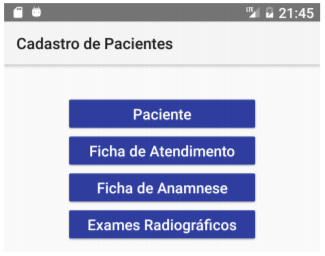
\includegraphics[scale=0.8]{cadastro-paciente}%% Dimensões e localização
% \fonte{}%% Fonte
% \end{figure}

\section{Implementação do sistema}
\label{sec:implementacaoSistema}

TODO

% Nesta seção é documentada a implementação do sistema com partes relevantes ou exemplos de código, rotinas, funções. Inclui, ainda, a descrição técnica do uso de recursos (componentes, bibliotecas, etc.) da linguagem. Ressalta-se que cada orientador avaliará juntamente com seu orientado o que poderá ser descrito nesta seção. Isso sem que sejam revelados detalhes do sistema que possam comprometer seu uso comercial ou científico ou que a descrição fique muito sucinta ou superficial.

% Em materiais e método estão quais os recursos utilizados, neste capítulo é reportado como esses recursos foram utilizados para resolver o problema.

% Sugere-se colocar listagens curtas de código, enfatizando aspectos específicos das tecnologias utilizadas ou da implementação. Sugere-se, ainda, que o código não seja apresentado sob a forma de print screen, e sim copiado e colado no texto, mantendo, se possível, a formatação. Todas as listagens de código devem ser devidamente explicadas. A explicação deve ser técnica, fundamentada em aspectos conceituais e boas práticas de programação.

% Enfatizar os diferenciais do sistema: procedimentos armazenados, consultas SQL, uso de componentes, uso de padrões de projeto, a forma de uso dos recursos da linguagem. Esses diferenciais são no sentido de explicitar as vantagens, desvantagens, dificuldades e facilidades que esses recursos impetraram no desenvolvimento do sistema em termos técnicos. Esses diferenciais servirão para avaliar pela utilização ou não desses recursos, pelo menos para sistemas iguais ou semelhantes ao reportado no trabalho.

% Reportar a forma como o sistema foi verificado e validado. No sentido de verificar se os requisitos definidos para o mesmo foram atendidos. Os testes podem ser realizados pelo professor orientador, pelos professores que compõem a banca, por pessoas que serviram de base para as informações para o sistema e etc. Os testes podem ser realizados com base em um plano de testes elaborado juntamente com a análise e projeto do sistema. Para validar a implementação podem ser desenvolvidas rotinas de teste unitário.

% Se houver implantação do sistema, mesmo que seja para teste, reportar a forma como isso foi feito, a geração de instaladores, os problemas com ambiente e sistema operacional, incluindo banco de dados e outros. Deixar explícito o procedimento para instalar e usar o sistema.

% Quando for necessário, citar no texto do trabalho nomes de campos, tabelas ou rotinas específicas utilizadas na implementação de um software, utilizar a fonte courier new para destacar esses nomes.

% Um exemplo de listagem de código fonte pode ser observado na \autoref{codigo:classeFoo}, que representa a classe Aluno.

% \begin{sourcecode}[htb]
% \caption{\label{codigo:classeFoo}Classe Aluno}
% \begin{lstlisting}[frame=single, language=Java]
% @Entity
% public class Foo {
 
%     @Id
%     @GeneratedValue(strategy = GenerationType.IDENTITY)
%     private Long id;
 
%     private String nome;
    
%     private Integer ra;
     
%     // constructor, getters and setters
% }
% \end{lstlisting}
% \fonte{}
% \end{sourcecode}

\section{Implantação do sistema}\label{sec:implantacaoSistema}

TODO

\section{Discussões}\label{sec:discussoes} 

TODO

% O trabalho contém esta seção quando considerado que há resultados (em termos de dados) e discussões relevantes ou suficientes para justificar uma seção. Se existentes e não justificarem uma seção, eles podem estar na seção que relata a implementação do sistema.

% Nesta seção estão os resultados obtidos da realização de testes quantitativos e qualitativos, independentemente da quantidade, tipo e volume de testes realizados. Os resultados dos testes são discutidos tendo como base o referencial teórico e os objetivos pretendidos com o trabalho. Esses testes podem resultar de implantação e testes de uso do sistema. 

\section{Trabalhos Relacionados}
\label{sec:trabalhosRelacionados}

O trabalho desenvolvido por \citet{qoselearning} realiza uma análise quantitativa do impacto de
parâmetros de conexão de rede em ambientes de ensino remoto sustentados por uma estrutura de \gls{vdi}.
A análise é feita a partir de um experimento com o objetivo de clarificar a relação entre a qualidade de
conexão com a internet e a usabilidade de sistemas de ensino remoto.

O resultado do experimento mostrou que é possível realizar atividades como escrita, desenhos e
consumo de mídias, sem grandes prejuízos para a usabilidade, mas é necessário que a conexão com a
internet tenha qualidade. Outro ponto importante é que fora atividades de visualização de vídeos, a
largura de banda não é um fator de grande consumo nesses tipos de ambientes.

Outro trabalho de grande relevância para essa produção, desenvolvido por \citet{edufirestick},
apresenta um sistema de \gls{vdi} para educação remota utilizando as mesmas tecnologias propostas
no presente trabalho. 

A proposta da produção é de criar uma \gls{vdi} de baixo custo com \glspl{ec2SpotInstance} da
\gls{aws} e com o \gls{guacamole} para gerenciamento das conexões, e permitindo o acesso de
qualquer dispositivo com um navegador de internet, até mesmo através televisões com acesso à internet,
como apresentado no trabalho.

A solução proposta por \citet{edufirestick} aborda um cenário de aula de laboratório, onde um
professor pode agendar um evento de criação das máquinas virtuais para os alunos e no horário da
aula, todos poderiam acessar o recurso reservado para a aula.

Em termos de custos operacionais, o trabalho apresenta uma estimativa de custo por usuário de
USD\$ 0.87 mensais com a utilização dos seguintes parâmetros:

\begin{itemize}
    \item Tempo de conexão diária: 18 horas
    \item Categoria da instância: t3.micro
    \item Sistema operacional: \textit{Microsoft Windows Server 2019}
    \item Memória: 4 GB de RAM
    \item Espaço em disco: 90 GB
    \item Região: São Paulo
\end{itemize}

Em termos de preço pela transferência de dados, o trabalho relata um custo de USD\$ 0.06 por hora em
picos onde o uso de banda chaga a 2 MB/s. O custo dos outros serviços que suportam a infraestrutura,
foi estimado em USD\$ 200.00 mensais.

O trabalho feito por \citet{edufirestick} apresenta um panorama muito promissor e consoante aos
objetivos do presente trabalho, demostrando que é possível executar a solução em um cenário de
laboratório. Mas ainda não apresenta resultados referentes ao gerenciamento de \glspl{desktop} que
tenham os dados persistidos, para outros cenários de uso, como o de pesquisa por exemplo.
% \part{Conclusão}
%%%% CAPÍTULO 5 - CONCLUSÕES E PERSPECTIVAS
%%
\chapter{Conclusão}\label{cap:conclusoeseperspectivas}

TODO
% Inicia com um resumo do trabalho, retomando o(s) objetivo(s), o referencial teórico e o uso das ferramentas e das tecnologias utilizadas no trabalho.

% A conclusão contém a opinião do autor em relação às vantagens, desvantagens, facilidades e limitações das tecnologias e/ou do método utilizados, as dificuldades encontradas e como foram superadas.

% Também devem ser apresentadas as vantagens, desvantagens e limitações do trabalho desenvolvido, sempre tendo em vista a sua contribuição para a comunidade acadêmica e profissional e para a sociedade como um todo.

% É a opinião técnica do autor do trabalho em relação ao assunto sob a forma de uma espécie de avaliação em relação ao trabalho desenvolvido e as tecnologias utilizadas.

% Finaliza verificando se o objetivo foi alcançado e com a opinião do autor sobre o assunto, de acordo com o referencial teórico e com os resultados obtidos.


\section{Perspectivas Futuras}\label{sec:perspectivasFuturas}

TODO

% As perspectivas futuras são opcionais, devem ser apresentadas somente caso o acadêmico pretenda dar continuidade ao trabalho, ou mesmo se ele julgar relevante que outras pessoas dêem continuidade ao seu trabalho.

%% Capítulos após este comando criam marcadores do pdf na raiz
% \phantompart%% Comente para remover este item


%% Formatação de páginas de elementos pós-textuais
\postextual%% Não comente esta linha

%% Arquivos de referências
\arquivosdereferencias{%% Arquivos bibtex sem a extensão .bib e separados por vírgula - Não comente esta linha
  %./PosTexto/exemplos-referencias,%% Arquivo de referências - Comente para remover este item
  main%% Arquivo de referências - Comente para remover este item
}%% Não comente esta linha

%% Glossário
\incluirglossario %% Comente para remover este item

%% Arquivos de apêndices
\begin{arquivosdeapendices}%% Os arquivos de apêndices devem se incluídos neste ambiente - Não comente esta linha
% \partapendices%% Página de início dos apêndices - adiciona uma página com o título Apêndices
%   %% Capítulo de exemplo
%%%% APÊNDICE A
%%
%% Texto ou documento elaborado pelo autor, a fim de complementar sua argumentação, sem prejuízo da unidade nuclear do trabalho.

%% Título e rótulo de apêndice (rótulos não devem conter caracteres especiais, acentuados ou cedilha)
\chapter{Relatório de Cobertura de Testes}
\label{cap:apendicea}

Este apêndice apresenta o relatório de cobertura de testes dos arquivos importados em casos de teste. A \autoref{tab:coberturaDosArquivosImportadosEmCasosDeTeste} apresenta a cobertura de linhas, funções e condicionais dos arquivos importados em casos de teste. Esses dados foram obtidos a partir do relatório gerado pelo \textit{framework} de testes Jest, que é utilizado para executar os testes automatizados do projeto.

É importante ressaltar que as estatísticas são calculadas com base nos arquivos que são importados em casos de testes. Portanto, arquivos não importados ficam de fora do cálculo.

O resultado acumulado da cobertura de linhas, funções e condicionais dos arquivos é de 1043/1117 (93.4\%), 218/244 (89.3\%) e 443/618 (71.7\%), respectivamente. Calculados a partir da execução de 131 casos de teste, distribuídos em 26 arquivos.

\begin{longtable}{@{\extracolsep{\fill}}p{0.45\linewidth}lll}%% Ambiente longtable
\caption{Cobertura dos arquivos importados em casos de teste\label{tab:coberturaDosArquivosImportadosEmCasosDeTeste}} \\%% Legenda e rótulo
\toprule
\textbf{Arquivo} & \textbf{Linhas} & \textbf{Funções} & \textbf{Condicionais} \\
\midrule
\endfirsthead%% Encerra cabeçalho da primeira página
\caption[]{Cobertura dos arquivos importados em casos de teste} \\%% Legenda
\multicolumn{4}{r}{\textbf{(continuação)}} \\
\toprule
\textbf{Arquivo} & \textbf{Linhas} & \textbf{Funções} & \textbf{Condicionais} \\
% \midrule
\endhead%% Encerra cabeçalho das demais páginas
% \midrule
\multicolumn{4}{r}{\textbf{(continua)}} \\
\endfoot%% Encerra rodapé das demais páginas
\bottomrule
\\[-0.5\linha]
\caption*{\nomefonte: Autoria própria (2024)} \\
\endlastfoot%% Encerra rodapé da última página

\_\_tests\_\_/fixtures/testDatabaseInstanceManager.ts & 11/17 (64.7\%) & 1/3 (33.3\%) & 0/1 (0.0\%) \\ \hline
packages/api/application/auth.ts & 25/25 (100.0\%) & 7/7 (100.0\%) & 1/4 (25.0\%) \\ \hline
packages/api/application/use-cases/instance/auto-turn-instance-off.ts & 13/13 (100.0\%) & 2/2 (100.0\%) & 7/11 (63.6\%) \\ \hline
packages/api/application/use-cases/instance/delete-instance.ts & 19/19 (100.0\%) & 2/2 (100.0\%) & 9/12 (75.0\%) \\ \hline
packages/api/application/use-cases/instance/get-instance-connection.ts & 37/37 (100.0\%) & 2/2 (100.0\%) & 17/20 (85.0\%) \\ \hline
packages/api/application/use-cases/instance/launch-instance.ts & 42/44 (95.5\%) & 2/2 (100.0\%) & 17/24 (70.8\%) \\ \hline
packages/api/application/use-cases/instance/link-launched-instance.ts & 23/23 (100.0\%) & 2/2 (100.0\%) & 8/11 (72.7\%) \\ \hline
packages/api/application/use-cases/instance/list-instances.ts & 25/25 (100.0\%) & 5/5 (100.0\%) & 12/15 (80.0\%) \\ \hline
packages/api/application/use-cases/instance/notify-instance-state-change.ts & 25/25 (100.0\%) & 2/2 (100.0\%) & 10/13 (76.9\%) \\ \hline
packages/api/application/use-cases/instance/reboot-instance.ts & 28/28 (100.0\%) & 2/2 (100.0\%) & 14/17 (82.4\%) \\ \hline
packages/api/application/use-cases/instance/schedule-instance-operation.ts & 8/8 (100.0\%) & 2/2 (100.0\%) & 5/8 (62.5\%) \\ \hline
packages/api/application/use-cases/instance/turn-instance-off.ts & 29/29 (100.0\%) & 2/2 (100.0\%) & 14/17 (82.4\%) \\ \hline
packages/api/application/use-cases/instance/turn-instance-on.ts & 29/29 (100.0\%) & 2/2 (100.0\%) & 14/17 (82.4\%) \\ \hline
packages/api/application/use-cases/instance/unschedule-instance-operation.ts & 8/8 (100.0\%) & 2/2 (100.0\%) & 5/8 (62.5\%) \\ \hline
packages/api/application/use-cases/instance-template/create-instance-template-from-instance.ts & 28/28 (100.0\%) & 2/2 (100.0\%) & 10/13 (76.9\%) \\ \hline
packages/api/application/use-cases/instance-template/create-instance-template.ts & 26/26 (100.0\%) & 2/2 (100.0\%) & 9/13 (69.2\%) \\ \hline
packages/api/application/use-cases/instance-template/delete-instance-template.ts & 18/19 (94.7\%) & 3/4 (75.0\%) & 6/9 (66.7\%) \\ \hline
packages/api/application/use-cases/instance-template/get-instance-template.ts & 15/15 (100.0\%) & 2/2 (100.0\%) & 6/9 (66.7\%) \\ \hline
packages/api/application/use-cases/instance-template/list-instance-templates.ts & 15/15 (100.0\%) & 2/2 (100.0\%) & 6/10 (60.0\%) \\ \hline
packages/api/application/use-cases/instance-template/update-instance-template.ts & 21/21 (100.0\%) & 3/3 (100.0\%) & 8/12 (66.7\%) \\ \hline
packages/api/application/use-cases/misc/list-instance-types.ts & 12/12 (100.0\%) & 2/2 (100.0\%) & 5/8 (62.5\%) \\ \hline
packages/api/application/use-cases/misc/list-recommended-machine-images.ts & 12/12 (100.0\%) & 2/2 (100.0\%) & 5/8 (62.5\%) \\ \hline
packages/api/application/use-cases/user/get-user.ts & 18/18 (100.0\%) & 2/2 (100.0\%) & 11/14 (78.6\%) \\ \hline
packages/api/application/use-cases/user/list-users.ts & 13/13 (100.0\%) & 2/2 (100.0\%) & 5/8 (62.5\%) \\ \hline
packages/api/application/use-cases/user/sign-in-user.ts & 14/14 (100.0\%) & 2/2 (100.0\%) & 7/10 (70.0\%) \\ \hline
packages/api/application/use-cases/user/sign-up-user.ts & 22/22 (100.0\%) & 2/2 (100.0\%) & 9/12 (75.0\%) \\ \hline
packages/api/application/use-cases/user/update-user-quotas.ts & 22/22 (100.0\%) & 4/4 (100.0\%) & 10/13 (76.9\%) \\ \hline
packages/api/application/use-cases/user/update-user-role.ts & 19/19 (100.0\%) & 2/2 (100.0\%) & 8/11 (72.7\%) \\ \hline
packages/api/domain/application-events/instance-connection-ended.ts & 6/6 (100.0\%) & 1/1 (100.0\%) & 0/0 (100.0\%) \\ \hline
packages/api/domain/application-events/instance-launched.ts & 8/8 (100.0\%) & 1/1 (100.0\%) & 0/0 (100.0\%) \\ \hline
packages/api/domain/application-events/instance-state-changed.ts & 8/8 (100.0\%) & 1/1 (100.0\%) & 0/0 (100.0\%) \\ \hline
packages/api/domain/decorators/use-case-execute.ts & 11/11 (100.0\%) & 3/3 (100.0\%) & 1/1 (100.0\%) \\ \hline
packages/api/domain/dtos/application-event.ts & 8/8 (100.0\%) & 2/2 (100.0\%) & 0/0 (100.0\%) \\ \hline
packages/api/domain/dtos/errors.ts & 21/23 (91.3\%) & 7/8 (87.5\%) & 16/18 (88.9\%) \\ \hline
packages/api/domain/dtos/instance-connection-type.ts & 2/2 (100.0\%) & 0/0 (100.0\%) & 0/0 (100.0\%) \\ \hline
packages/api/domain/dtos/instance-platform.ts & 2/2 (100.0\%) & 0/0 (100.0\%) & 0/0 (100.0\%) \\ \hline
packages/api/domain/dtos/instance-state.ts & 2/2 (100.0\%) & 0/0 (100.0\%) & 0/0 (100.0\%) \\ \hline
packages/api/domain/dtos/principal.ts & 2/2 (100.0\%) & 0/0 (100.0\%) & 0/0 (100.0\%) \\ \hline
packages/api/domain/dtos/role.ts & 2/2 (100.0\%) & 0/0 (100.0\%) & 0/0 (100.0\%) \\ \hline
packages/api/domain/dtos/seek-paginated.ts & 2/2 (100.0\%) & 0/0 (100.0\%) & 0/0 (100.0\%) \\ \hline
packages/api/domain/dtos/virtual-instance-type.ts & 2/2 (100.0\%) & 0/0 (100.0\%) & 0/0 (100.0\%) \\ \hline
packages/api/domain/entities/instance-template.ts & 31/34 (91.2\%) & 8/9 (88.9\%) & 2/9 (22.2\%) \\ \hline
packages/api/domain/entities/instance.ts & 44/47 (93.6\%) & 16/17 (94.1\%) & 16/21 (76.2\%) \\ \hline
packages/api/domain/entities/user.ts & 33/36 (91.7\%) & 10/11 (90.9\%) & 15/21 (71.4\%) \\ \hline
packages/api/infrastructure/auth/in-memory-auth.ts & 7/7 (100.0\%) & 2/2 (100.0\%) & 5/6 (83.3\%) \\ \hline
packages/api/infrastructure/config-vault/in-memory-config-vault.ts & 4/4 (100.0\%) & 2/2 (100.0\%) & 0/1 (0.0\%) \\ \hline
packages/api/infrastructure/connection-encoder/guacamole-connection-encoder.ts & 18/18 (100.0\%) & 4/4 (100.0\%) & 0/1 (0.0\%) \\ \hline
packages/api/infrastructure/event-publisher/in-memory-event-publisher.ts & 7/9 (77.8\%) & 4/4 (100.0\%) & 3/4 (75.0\%) \\ \hline
packages/api/infrastructure/instance-repository/in-memory-instance-repository.ts & 53/59 (89.8\%) & 22/23 (95.7\%) & 36/48 (75.0\%) \\ \hline
packages/api/infrastructure/instance-template-repository/in-memory-instance-template-repository.ts & 39/45 (86.7\%) & 15/16 (93.8\%) & 27/35 (77.1\%) \\ \hline
packages/api/infrastructure/logger/in-memory-logger.ts & 12/14 (85.7\%) & 5/7 (71.4\%) & 1/1 (100.0\%) \\ \hline
packages/api/infrastructure/user-repository/in-memory-user-repository.ts & 35/52 (67.3\%) & 12/22 (54.5\%) & 17/35 (48.6\%) \\ \hline
packages/api/infrastructure/virtualization-gateway/in-memory-virtualization-gateway.ts & 107/128 (83.6\%) & 36/41 (87.8\%) & 66/89 (74.2\%) \\


\end{longtable}


% Quando houver necessidade pode-se apresentar como apêndice documento(s) auxiliar(es) e/ou complementar(es) como: legislação, estatutos, gráficos, tabelas, etc. Os apêndices são enumerados com letras maiúsculas: \autoref{cap:apendicea}, \autoref{cap:apendiceb}, etc.

% No \latex\ apêndices são editados como capítulos. O comando \verb|\appendix| faz com que todos os capítulos seguintes sejam considerados apêndices.

% Apêndices complementam o texto principal da tese com informações para leitores com especial interesse no tema, devendo ser considerados leitura opcional, ou seja, o entendimento do texto principal da tese não deve exigir a leitura atenta dos apêndices.

% Apêndices usualmente contemplam provas de teoremas, deduções de fórmulas matemáticas, diagramas esquemáticos, gráficos e trechos de código. Quanto a este último, código extenso não deve fazer parte da tese, mesmo como apêndice. O ideal é disponibilizar o código na Internet para os interessados em examiná-lo ou utilizá-lo.

%% Título e rótulo de seção (rótulos não devem conter caracteres especiais, acentuados ou cedilha)
%\section{Título da Seção Secundária do Apêndice B}\label{sec:secaoapendicea}

%Exemplo de seção secundária em apêndice (\autoref{sec:secaoapendicea} do \autoref{cap:apendicea}).

%% Título e rótulo de seção (rótulos não devem conter caracteres especiais, acentuados ou cedilha)
%\subsection{Título da Seção Terciária do Apêndice B}\label{subsec:subsecaoapendicea}

%Exemplo de seção terciária em apêndice (\autoref{subsec:subsecaoapendicea} do \autoref{cap:apendicea}).

%% Título e rótulo de seção (rótulos não devem conter caracteres especiais, acentuados ou cedilha)
%\subsubsection{Título da seção quaternária do Apêndice B}\label{subsubsec:subsubsecaoapendicea}

%Exemplo de seção quaternária em apêndice (\autoref{subsubsec:subsubsecaoapendicea} do \autoref{cap:apendicea}).

%% Título e rótulo de seção (rótulos não devem conter caracteres especiais, acentuados ou cedilha)
%\paragraph{Título da seção quinária do Apêndice B}\label{para:paragraphapendicea}

%Exemplo de seção quinária em apêndice (\autoref{para:paragraphapendicea} do \autoref{cap:apendicea}).%% Apêndice - Comente para remover este item
%%%% APÊNDICE B
%%
%% Texto ou documento elaborado pelo autor, a fim de complementar sua argumentação, sem prejuízo da unidade nuclear do trabalho.

%% Título e rótulo de apêndice (rótulos não devem conter caracteres especiais, acentuados ou cedilha)
\chapter{Código Fonte do Fluxo de Integração Contínua}\label{cap:apendiceb}

O código da \autoref{codigo:ciyaml} apresenta as etapas que compõem o fluxo de integração contínua do projeto. O arquivo é escrito em \textit{YAML} e é responsável por automatizar a execução de tarefas como instalação de dependências, execução de testes, análise estática de código e envio de relatórios de cobertura de testes para o serviço de terceiros \textit{Codecov}, que é um serviço de acompanhamento de cobertura de testes.

\begin{sourcecode}[htb]
\caption{\label{codigo:ciyaml}Arquivo de configuração do fluxo de integração contínua}
\begin{lstlisting}[frame=single]
name: CI

on: ['push', 'pull_request']

concurrency:
    group: '${{ github.workflow }}-
        ${{ github.event.pull_request.number || github.ref }}'
    cancel-in-progress: true

jobs:
    continuous-integration:
    runs-on: ubuntu-latest
    steps:
        - name: Checkout
        uses: actions/checkout@v4
        with:
            fetch-depth: 0

        - name: Setup Node.js
        uses: actions/setup-node@v4
        with:
            node-version-file: '.nvmrc'
            cache: 'npm'
            cache-dependency-path: |
            package-lock.json
            packages/*/package-lock.json

        - name: Install dependencies, typecheck, lint, format, test
        run: |
            npm ci
            npm run typecheck
            npm run lint
            npx prettier --check .
            npx jest --ci --coverage
        env:
            CI: true

        - name: Upload coverage reports to Codecov
        uses: codecov/codecov-action@v4.0.1
        with:
            token: ${{ secrets.CODECOV_TOKEN }}
    
\end{lstlisting}
\fonte{}
\end{sourcecode}%% Apêndice - Comente para remover este item
\end{arquivosdeapendices}%% Não comente esta linha


% \begin{apendicesenv}%% Ambiente apendicesenv

% \partapendices
% \chapter{Ola}

% \lipsum[55-56]

% \end{apendicesenv}

%% Arquivos de anexos
\begin{arquivosdeanexos}%% Os arquivos de anexos devem se incluídos neste ambiente - Não comente esta linha
  %\partanexos%% Página de início dos anexos - adiciona uma página com o título Anexos

  % %%%% ANEXO A
%%
%% Texto ou documento não elaborado pelo autor, que serve de fundamentação, comprovação e ilustração.

%% Título e rótulo de anexo (rótulos não devem conter caracteres especiais, acentuados ou cedilha)
\anexos
\chapter{Direitos Autorais - Lei N\texorpdfstring{.\textsuperscript{o}}{o.} 9.610, de 19 de Fevereiro de 1998: Disposições Preliminares}\label{cap:anexoa}

\centerline{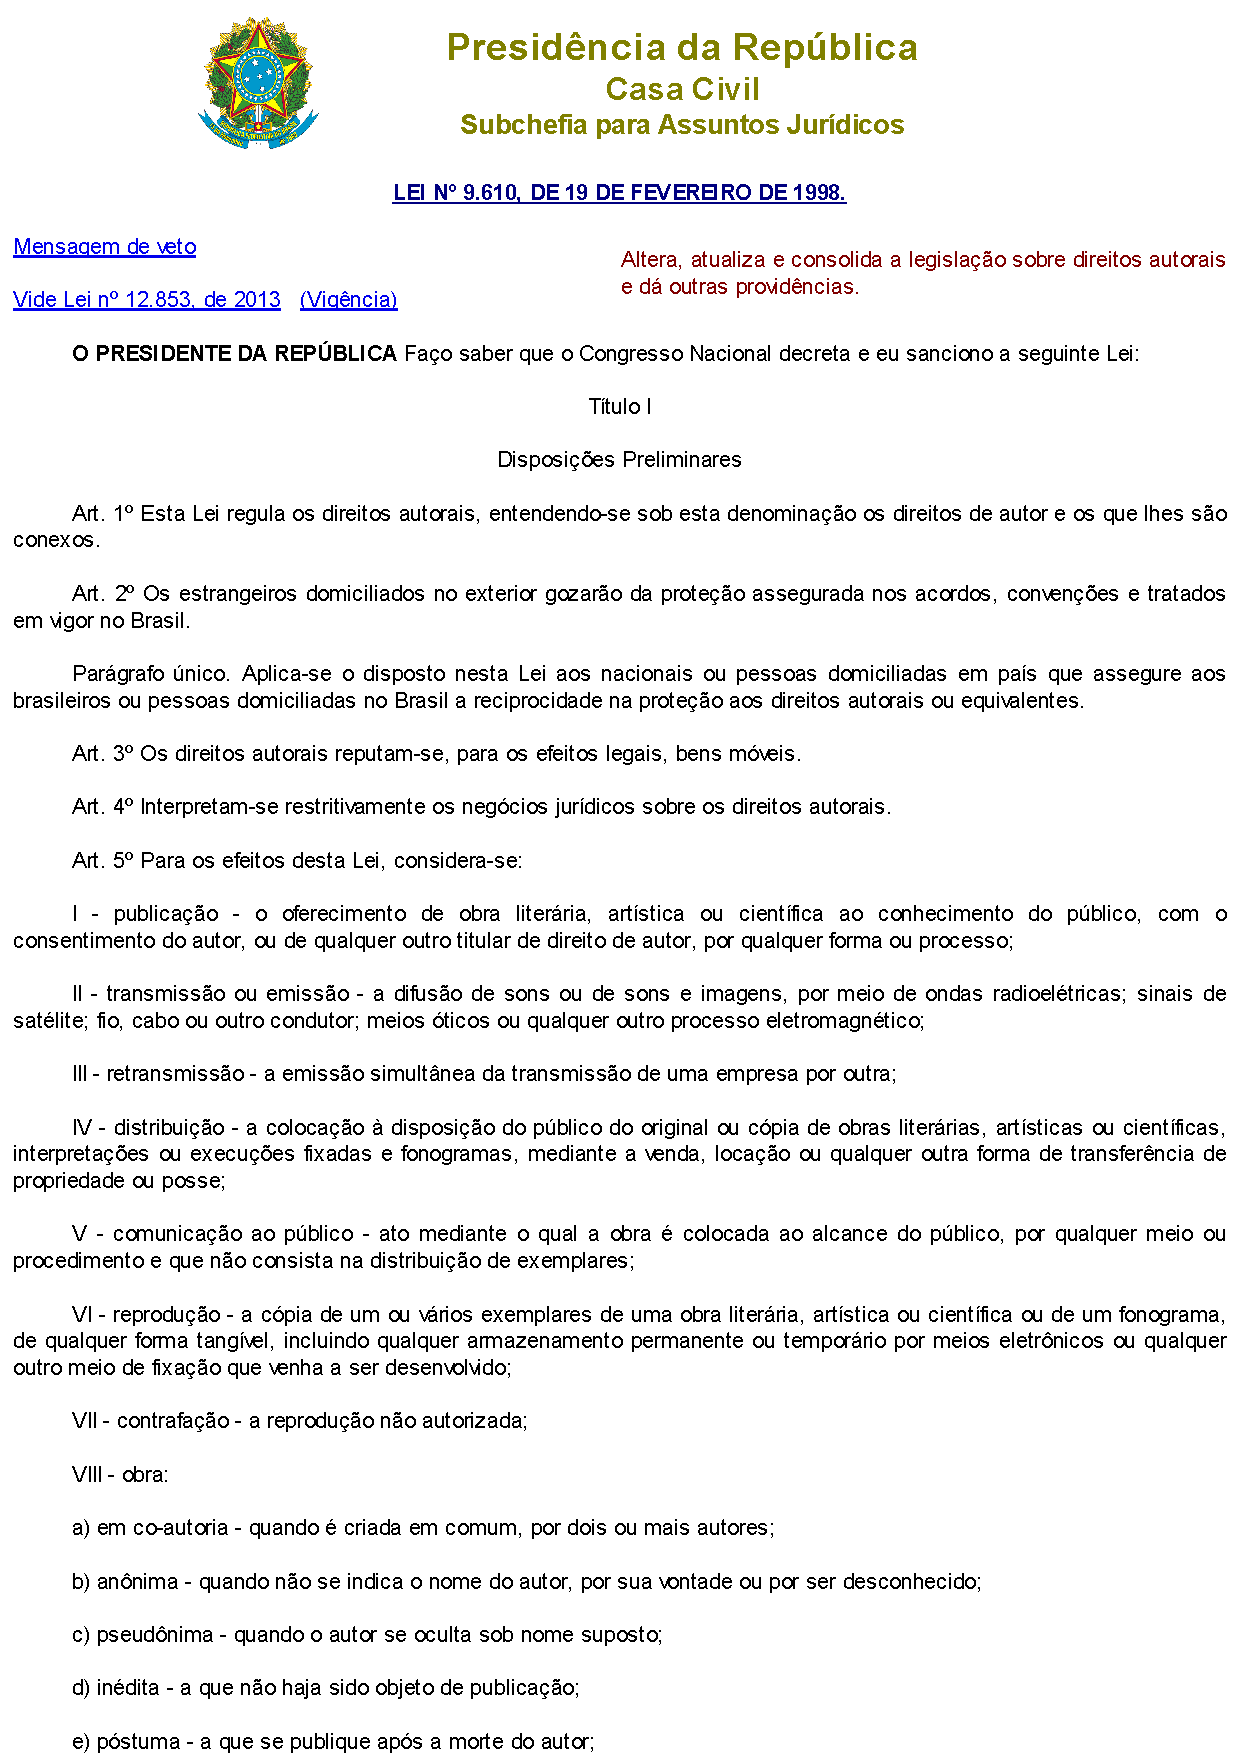
\includegraphics[width=\textwidth]{./PosTexto/Ilustracoes/lei-n9610-p1}}%% Imagem (Dimensões e localização)

\centerline{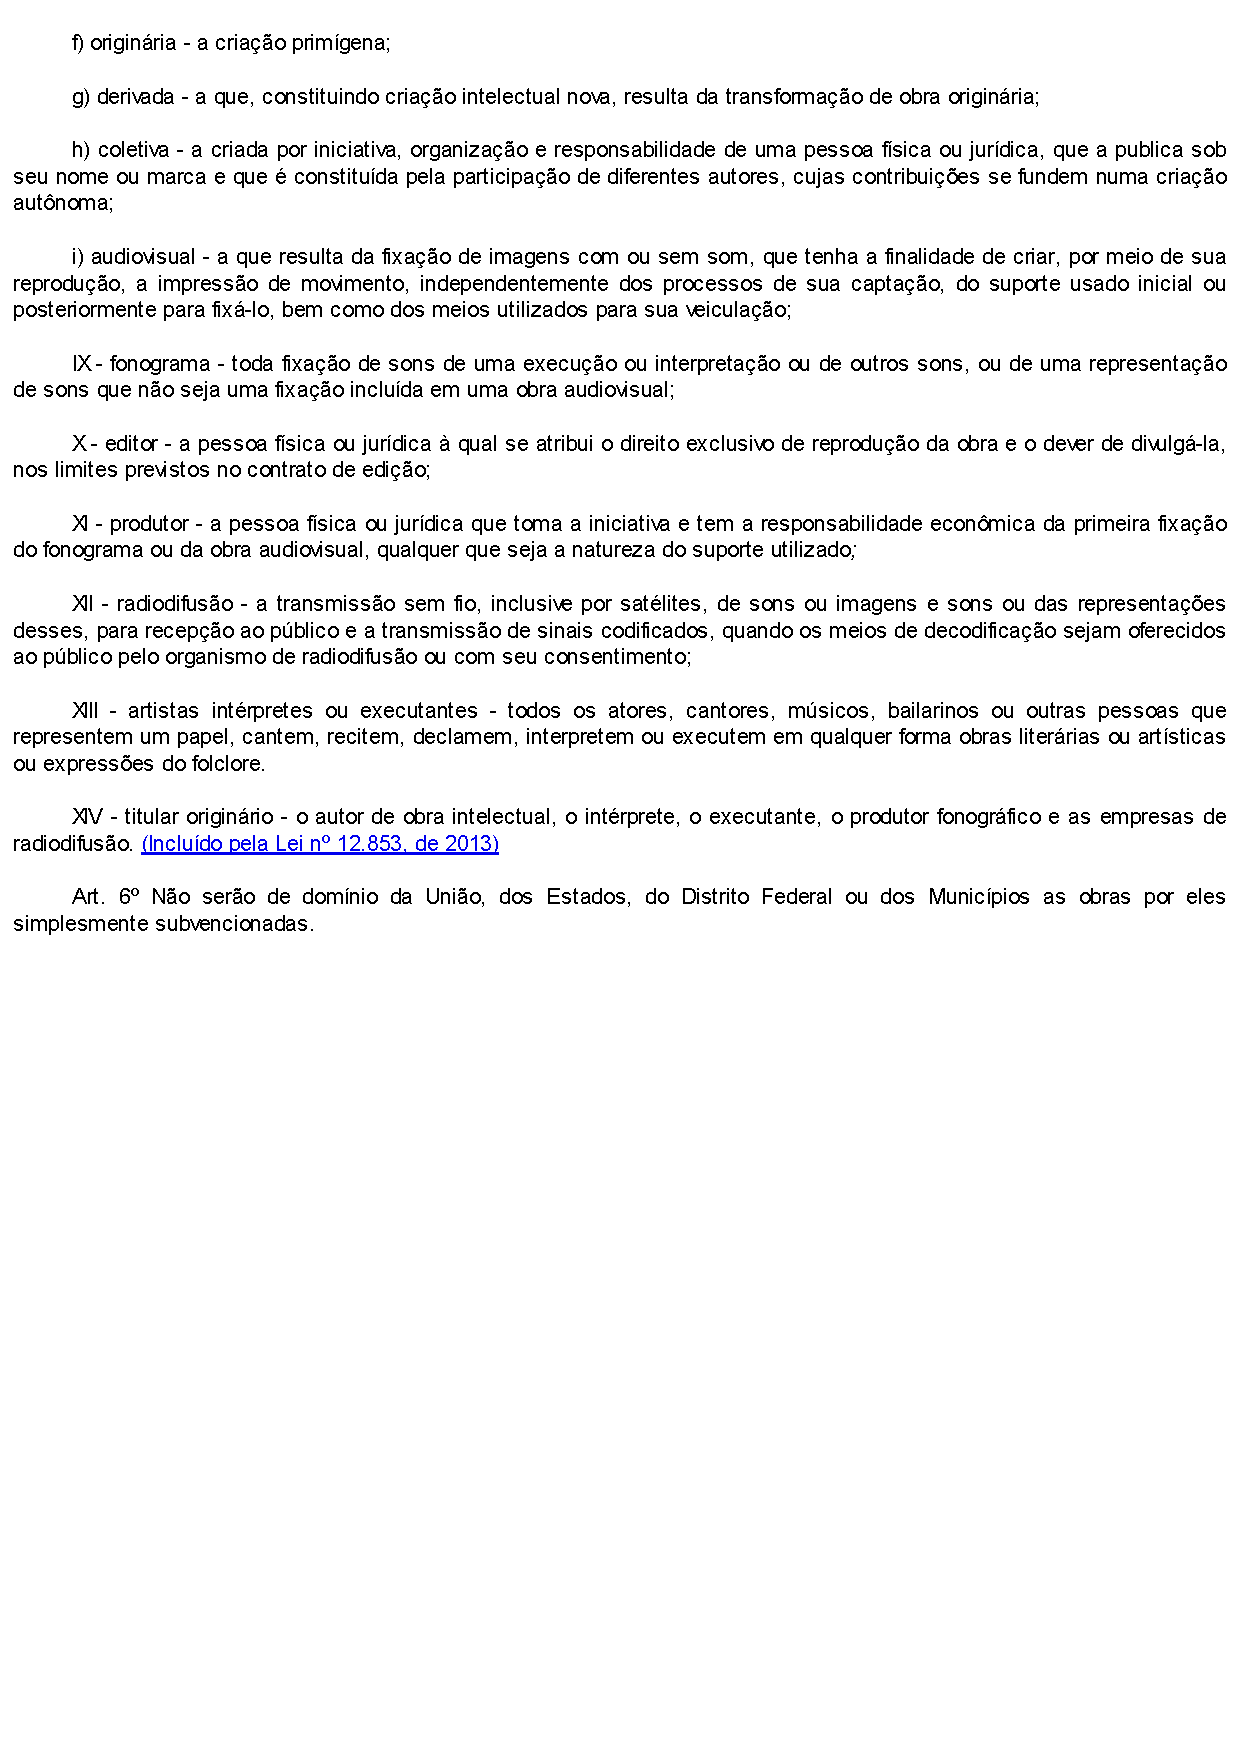
\includegraphics[width=\textwidth]{./PosTexto/Ilustracoes/lei-n9610-p2}}%% Imagem (Dimensões e localização)
%% Anexo - Comente para remover este item
  % %%%% ANEXO B
%%
%% Texto ou documento não elaborado pelo autor, que serve de fundamentação, comprovação e ilustração.

%% Título e rótulo de anexo (rótulos não devem conter caracteres especiais, acentuados ou cedilha)
\chapter{Normas para Elaboração de Trabalhos Acadêmicos}\label{cap:anexob}

As normas da \gls{utfpr} podem ser acessadas em: \url{http://portal.utfpr.edu.br/biblioteca/trabalhos-academicos/discentes/orientacao-para-trabalhos-academicos}. Ver Figura \ref{fig:capadolivro}.

\begin{figure}[htb]%% Ambiente figure
\captionsetup{width=0.9\textwidth}%% Largura da legenda
\caption{Sítio: Normas para Elaboração de Trabalhos Acadêmicos.}%% Legenda
\label{fig:capadolivro}%% Rótulo
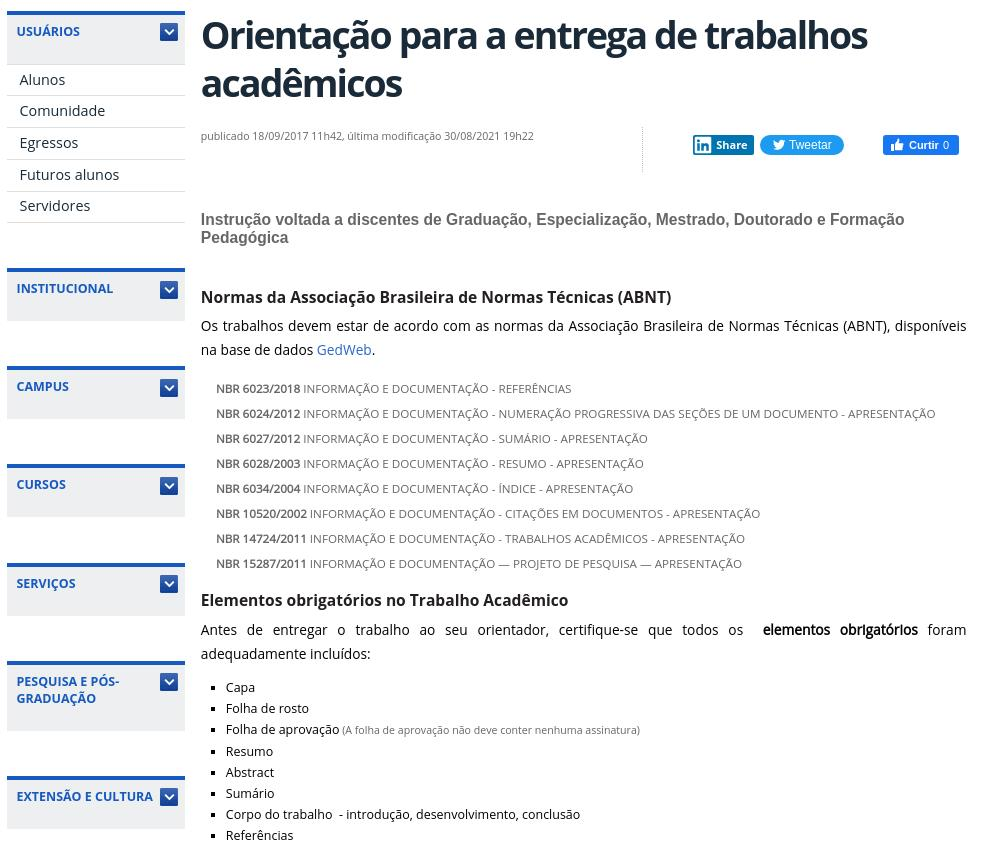
\includegraphics[width=0.9\textwidth]{normas}%% Dimensões e localização
\fonte{\cite{UTFPR2008}}%% Fonte
\end{figure}

%% Anexo - Comente para remover este item
\end{arquivosdeanexos}%% Não comente esta linha

%% Índice - Adiciona um índice remissivo.
%\incluirindice%% Comente para remover este item

%% Fim do documento
\end{document}%% Não comente esta linha
